% Generated by genfigs.py (V31) -- all coordinates computed from exact formulas.
\usepackage{tikz}
\usetikzlibrary{calc,arrows.meta,decorations.pathreplacing,backgrounds}
% Unified V31 editorial palette
\definecolor{ink}{RGB}{28,36,48}
\definecolor{supp}{RGB}{22,82,158}
\definecolor{trans}{RGB}{21,128,82}
\definecolor{acc}{RGB}{210,88,18}
\definecolor{tealc}{RGB}{13,132,148}
\definecolor{plum}{RGB}{128,42,138}
\definecolor{slatec}{RGB}{110,124,142}
\definecolor{rectfill}{RGB}{246,249,253}
\definecolor{trifill}{RGB}{254,242,230}
\definecolor{bluefill}{RGB}{236,244,252}
\definecolor{greenfill}{RGB}{236,249,242}
\definecolor{chainc}{RGB}{168,178,192}
\definecolor{chainp}{RGB}{198,142,146}
\definecolor{faint}{RGB}{204,212,222}
\definecolor{gridc}{RGB}{226,232,240}
\tikzset{
  rect/.style={line width=0.95pt,ink},
  rectbg/.style={fill=rectfill},
  chain/.style={line width=0.42pt,chainc},
  chainpar/.style={line width=0.48pt,chainp},
  chainfaint/.style={line width=0.35pt,faint},
  support/.style={line width=1.6pt,supp},
  transport/.style={line width=1.15pt,trans},
  accent/.style={line width=1.35pt,acc},
  aux/.style={line width=0.5pt,densely dashed,slatec!75},
  pt/.style={circle,fill=ink,draw=white,line width=0.45pt,inner sep=1.45pt},
  ptsm/.style={circle,fill=ink,draw=white,line width=0.35pt,inner sep=1.15pt},
  ptacc/.style={circle,fill=acc,draw=white,line width=0.45pt,inner sep=1.55pt},
  ptsupp/.style={circle,fill=supp,draw=white,line width=0.45pt,inner sep=1.55pt},
  pttrans/.style={circle,fill=trans,draw=white,line width=0.45pt,inner sep=1.55pt},
  lab/.style={font=\small,text=ink,inner sep=1.8pt},
  labsm/.style={font=\footnotesize,text=ink,inner sep=1.4pt},
  halo/.style={fill=white,fill opacity=0.88,text opacity=1,rounded corners=1pt,inner sep=1.2pt},
  ttl/.style={font=\small\bfseries,text=ink,anchor=west},
  badge/.style={circle,fill=supp,text=white,font=\scriptsize\bfseries,inner sep=1.2pt,minimum size=11pt},
  badgeacc/.style={circle,fill=acc,text=white,font=\scriptsize\bfseries,inner sep=1.2pt,minimum size=11pt},
  badgetrans/.style={circle,fill=trans,text=white,font=\scriptsize\bfseries,inner sep=1.2pt,minimum size=11pt},
  dim/.style={line width=0.55pt,ink!80,{Latex[length=4pt]}-{Latex[length=4pt]}},
  card/.style={draw=slatec!40,fill=rectfill,rounded corners=3pt,line width=0.5pt},
}

\newcommand{\figAnatomy}{%
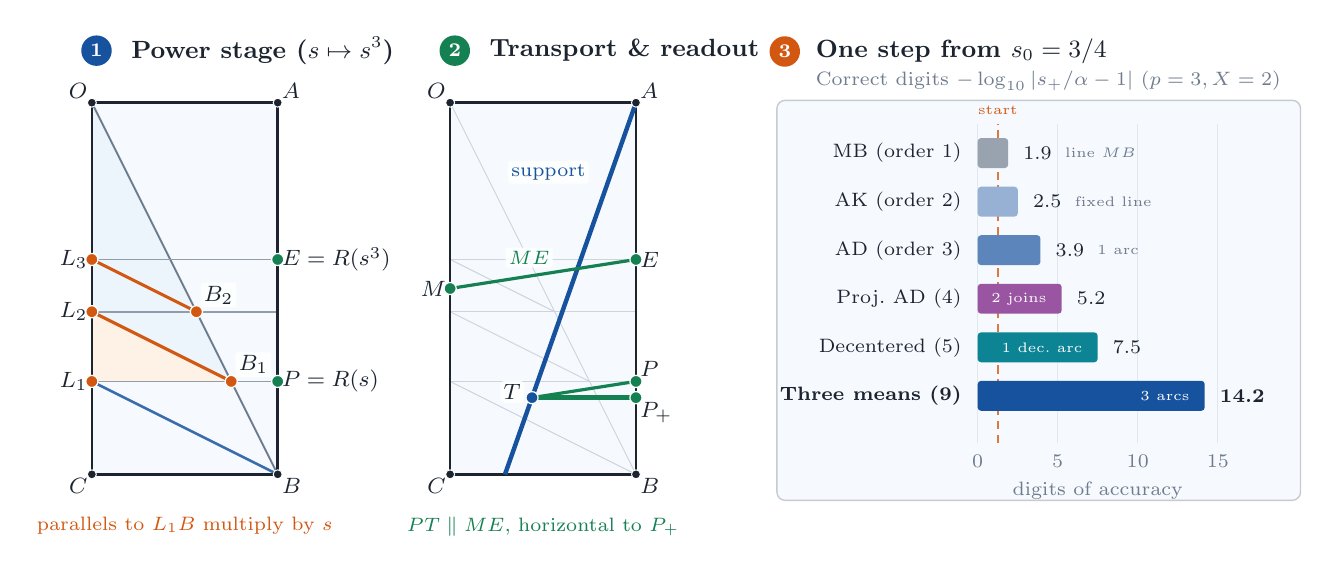
\begin{tikzpicture}
\begin{scope}[shift={(0,0)},scale=1.18]
\node[badge] at (0.05,4.560) {1};
\node[ttl] at (0.32,4.560) {Power stage ($s \mapsto s^3$)};
\fill[rectbg] (0.0000,0.0000) rectangle (2.0000,4.0000);
\fill[bluefill] (0.0000,4.0000)--(0.0000,1.0000)--(1.5000,1.0000)--cycle;
\fill[trifill] (0.0000,1.0000)--(0.0000,1.7500)--(1.5000,1.0000)--cycle;
\draw[line width=0.7pt,slatec] (0.0000,4.0000)--(2.0000,0.0000);
\draw[line width=0.9pt,supp!85] (0.0000,1.0000)--(2.0000,0.0000);
\draw[line width=0.6pt,slatec!75] (0,1.0000)--(2.0,1.0000);
\draw[line width=0.6pt,slatec!75] (0,1.7500)--(2.0,1.7500);
\draw[line width=0.6pt,slatec!75] (0,2.3125)--(2.0,2.3125);
\draw[line width=1.1pt,acc] (1.5000,1.0000)--(0.0000,1.7500);
\draw[line width=1.1pt,acc] (1.1250,1.7500)--(0.0000,2.3125);
\draw[rect] (0.0000,0.0000) rectangle (2.0000,4.0000);
\node[ptsm] at (0.0000,4.0000) {};
\node[ptsm] at (2.0000,4.0000) {};
\node[ptsm] at (0.0000,0.0000) {};
\node[ptsm] at (2.0000,0.0000) {};
\node[ptacc] at (0.0000,1.0000) {};
\node[ptacc] at (0.0000,1.7500) {};
\node[ptacc] at (0.0000,2.3125) {};
\node[ptacc] at (1.5000,1.0000) {};
\node[ptacc] at (1.1250,1.7500) {};
\node[pttrans] at (2.0000,1.0000) {};
\node[pttrans] at (2.0000,2.3125) {};
\node[labsm,above left] at (0.0000,4.0000) {$O$};
\node[labsm,above right] at (2.0000,4.0000) {$A$};
\node[labsm,below left] at (0.0000,0.0000) {$C$};
\node[labsm,below right] at (2.0000,0.0000) {$B$};
\node[labsm,left] at (0.0000,1.0000) {$L_1$};
\node[labsm,left] at (0.0000,1.7500) {$L_2$};
\node[labsm,left] at (0.0000,2.3125) {$L_3$};
\node[labsm,halo,above right] at (1.5400,1.0400) {$B_1$};
\node[labsm,halo,above right] at (1.1650,1.7900) {$B_2$};
\node[labsm,right] at (2.0000,1.0000) {$P=R(s)$};
\node[labsm,right] at (2.0000,2.3125) {$E=R(s^3)$};
\node[font=\scriptsize,text=acc,anchor=north] at (1.000,-0.35) {parallels to $L_1B$ multiply by $s$};
\end{scope}
\begin{scope}[shift={(4.55,0)},scale=1.18]
\node[badgetrans] at (0.05,4.560) {2};
\node[ttl] at (0.32,4.560) {Transport \& readout};
\fill[rectbg] (0.0000,0.0000) rectangle (2.0000,4.0000);
\draw[chainfaint] (0.0000,4.0000)--(2.0000,0.0000);
\draw[chainfaint] (0.0000,1.0000)--(2.0000,0.0000);
\draw[chainfaint] (0,1.0000)--(2.0,1.0000);
\draw[chainfaint] (0,1.7500)--(2.0,1.7500);
\draw[chainfaint] (0,2.3125)--(2.0,2.3125);
\draw[chainfaint] (1.5000,1.0000)--(0.0000,1.7500);
\draw[chainfaint] (1.1250,1.7500)--(0.0000,2.3125);
\draw[rect] (0.0000,0.0000) rectangle (2.0000,4.0000);
\draw[support] (2.0000,4.0000)--(0.5905,0.0000);
\draw[transport] (0.0000,2.0000)--(2.0000,2.3125);
\draw[transport] (2.0000,1.0000)--(0.8813,0.8252);
\draw[transport,line width=1.65pt] (0.8813,0.8252)--(2.0000,0.8252);
\node[ptsm] at (0.0000,4.0000) {};
\node[ptsm] at (2.0000,4.0000) {};
\node[ptsm] at (0.0000,0.0000) {};
\node[ptsm] at (2.0000,0.0000) {};
\node[pttrans] at (0.0000,2.0000) {};
\node[pttrans] at (2.0000,2.3125) {};
\node[pttrans] at (2.0000,1.0000) {};
\node[pttrans] at (2.0000,0.8252) {};
\node[ptsupp] at (0.8813,0.8252) {};
\node[labsm,above left] at (0.0000,4.0000) {$O$};
\node[labsm,above right] at (2.0000,4.0000) {$A$};
\node[labsm,below left] at (0.0000,0.0000) {$C$};
\node[labsm,below right] at (2.0000,0.0000) {$B$};
\node[labsm,left] at (0.0000,2.0000) {$M$};
\node[labsm,right] at (2.0000,2.3125) {$E$};
\node[labsm,above right] at (2.0000,1.0000) {$P$};
\node[labsm,below right] at (2.0000,0.8252) {$P_+$};
\node[labsm,halo,left] at (0.8013,0.8852) {$T$};
\node[font=\scriptsize,text=supp,halo,anchor=east] at (1.50,3.25) {support};
\node[font=\scriptsize,text=trans,halo,anchor=south] at (0.85,2.22) {$ME$};
\node[font=\scriptsize,text=trans,anchor=north] at (1.000,-0.35) {$PT \parallel ME$, horizontal to $P_+$};
\end{scope}
\begin{scope}[shift={(8.95,0.35)}]
\node[badgeacc] at (-0.15,5.020) {3};
\node[ttl] at (0.12,5.020) {One step from $s_0=3/4$};
\node[font=\scriptsize,text=slatec,anchor=west] at (0.12,4.650) {Correct digits $-\log_{10}|s_+/\alpha-1|$ ($p=3, X=2$)};
\draw[card] (-0.25,-0.68) rectangle (6.40,4.40);
\draw[line width=0.35pt,gridc] (2.300,0.05)--(2.300,4.100);
\node[font=\scriptsize,text=slatec] at (2.300,-0.18) {0};
\draw[line width=0.35pt,gridc] (3.317,0.05)--(3.317,4.100);
\node[font=\scriptsize,text=slatec] at (3.317,-0.18) {5};
\draw[line width=0.35pt,gridc] (4.333,0.05)--(4.333,4.100);
\node[font=\scriptsize,text=slatec] at (4.333,-0.18) {10};
\draw[line width=0.35pt,gridc] (5.350,0.05)--(5.350,4.100);
\node[font=\scriptsize,text=slatec] at (5.350,-0.18) {15};
\draw[line width=0.6pt,densely dashed,acc!80] (2.556,0.05)--(2.556,4.100);
\node[font=\tiny,text=acc,anchor=south] at (2.556,4.100) {start};
\fill[slatec!70,rounded corners=1.2pt] (2.300,3.540) rectangle (2.687,3.920);
\node[font=\scriptsize,text=ink,anchor=east] at (2.220,3.730) {MB (order 1)};
\node[font=\scriptsize,text=ink,anchor=west] at (2.757,3.730) {1.9};
\node[font=\tiny,text=slatec,anchor=west] at (3.287,3.730) {line $MB$};
\fill[supp!45,rounded corners=1.2pt] (2.300,2.923) rectangle (2.809,3.303);
\node[font=\scriptsize,text=ink,anchor=east] at (2.220,3.113) {AK (order 2)};
\node[font=\scriptsize,text=ink,anchor=west] at (2.879,3.113) {2.5};
\node[font=\tiny,text=slatec,anchor=west] at (3.409,3.113) {fixed line};
\fill[supp!70,rounded corners=1.2pt] (2.300,2.307) rectangle (3.097,2.687);
\node[font=\scriptsize,text=ink,anchor=east] at (2.220,2.497) {AD (order 3)};
\node[font=\scriptsize,text=ink,anchor=west] at (3.167,2.497) {3.9};
\node[font=\tiny,text=slatec,anchor=west] at (3.697,2.497) {1 arc};
\fill[plum!80,rounded corners=1.2pt] (2.300,1.690) rectangle (3.367,2.070);
\node[font=\scriptsize,text=ink,anchor=east] at (2.220,1.880) {Proj.\ AD (4)};
\node[font=\scriptsize,text=ink,anchor=west] at (3.437,1.880) {5.2};
\node[font=\tiny,text=white,anchor=east] at (3.297,1.880) {2 joins};
\fill[tealc,rounded corners=1.2pt] (2.300,1.073) rectangle (3.823,1.453);
\node[font=\scriptsize,text=ink,anchor=east] at (2.220,1.263) {Decentered (5)};
\node[font=\scriptsize,text=ink,anchor=west] at (3.893,1.263) {7.5};
\node[font=\tiny,text=white,anchor=east] at (3.753,1.263) {1 dec.\ arc};
\fill[supp,rounded corners=1.2pt] (2.300,0.457) rectangle (5.183,0.837);
\node[font=\scriptsize\bfseries,text=ink,anchor=east] at (2.220,0.647) {Three means (9)};
\node[font=\scriptsize\bfseries,text=ink,anchor=west] at (5.253,0.647) {14.2};
\node[font=\tiny,text=white,anchor=east] at (5.113,0.647) {3 arcs};
\node[font=\scriptsize,text=slatec,anchor=north] at (3.825,-0.32) {digits of accuracy};
\end{scope}
\end{tikzpicture}%
}

\newcommand{\figTarget}{%
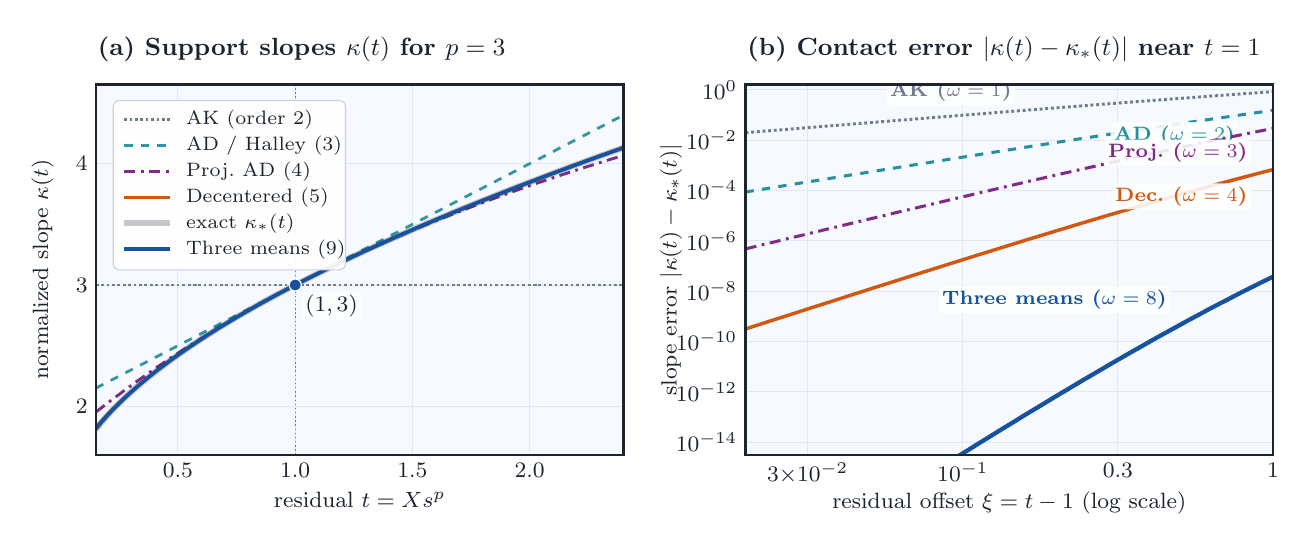
\begin{tikzpicture}
\begin{scope}[shift={(0,0)}]
\node[ttl] at (-0.1,5.150) {(a) Support slopes $\kappa(t)$ for $p=3$};
\fill[rectbg] (0,0) rectangle (6.700,4.700);
\draw[line width=0.35pt,gridc] (1.042,0)--(1.042,4.700);
\node[labsm,below] at (1.042,-0.05) {0.5};
\draw[line width=0.35pt,gridc] (2.531,0)--(2.531,4.700);
\node[labsm,below] at (2.531,-0.05) {1.0};
\draw[line width=0.35pt,gridc] (4.020,0)--(4.020,4.700);
\node[labsm,below] at (4.020,-0.05) {1.5};
\draw[line width=0.35pt,gridc] (5.509,0)--(5.509,4.700);
\node[labsm,below] at (5.509,-0.05) {2.0};
\draw[line width=0.35pt,gridc] (0,0.616)--(6.700,0.616);
\node[labsm,left] at (-0.05,0.616) {2};
\draw[line width=0.35pt,gridc] (0,2.157)--(6.700,2.157);
\node[labsm,left] at (-0.05,2.157) {3};
\draw[line width=0.35pt,gridc] (0,3.698)--(6.700,3.698);
\node[labsm,left] at (-0.05,3.698) {4};
\draw[line width=0.5pt,densely dotted,slatec] (2.531,0)--(2.531,4.700);
\begin{scope}
\clip (0,0) rectangle (6.700,4.700);
\draw[slatec,line width=0.95pt,densely dotted] (0.000,2.157)--(0.074,2.157)--(0.149,2.157)--(0.223,2.157)--(0.298,2.157)--(0.372,2.157)--(0.447,2.157)--(0.521,2.157)--(0.596,2.157)--(0.670,2.157)--(0.744,2.157)--(0.819,2.157)--(0.893,2.157)--(0.968,2.157)--(1.042,2.157)--(1.117,2.157)--(1.191,2.157)--(1.266,2.157)--(1.340,2.157)--(1.414,2.157)--(1.489,2.157)--(1.563,2.157)--(1.638,2.157)--(1.712,2.157)--(1.787,2.157)--(1.861,2.157)--(1.936,2.157)--(2.010,2.157)--(2.084,2.157)--(2.159,2.157)--(2.233,2.157)--(2.308,2.157)--(2.382,2.157)--(2.457,2.157)--(2.531,2.157)--(2.606,2.157)--(2.680,2.157)--(2.754,2.157)--(2.829,2.157)--(2.903,2.157)--(2.978,2.157)--(3.052,2.157)--(3.127,2.157)--(3.201,2.157)--(3.276,2.157)--(3.350,2.157)--(3.424,2.157)--(3.499,2.157)--(3.573,2.157)--(3.648,2.157)--(3.722,2.157)--(3.797,2.157)--(3.871,2.157)--(3.946,2.157)--(4.020,2.157)--(4.094,2.157)--(4.169,2.157)--(4.243,2.157)--(4.318,2.157)--(4.392,2.157)--(4.467,2.157)--(4.541,2.157)--(4.616,2.157)--(4.690,2.157)--(4.764,2.157)--(4.839,2.157)--(4.913,2.157)--(4.988,2.157)--(5.062,2.157)--(5.137,2.157)--(5.211,2.157)--(5.286,2.157)--(5.360,2.157)--(5.434,2.157)--(5.509,2.157)--(5.583,2.157)--(5.658,2.157)--(5.732,2.157)--(5.807,2.157)--(5.881,2.157)--(5.956,2.157)--(6.030,2.157)--(6.104,2.157)--(6.179,2.157)--(6.253,2.157)--(6.328,2.157)--(6.402,2.157)--(6.477,2.157)--(6.551,2.157)--(6.626,2.157)--(6.700,2.157);
\draw[tealc!85,line width=1.0pt,dashed] (0.000,0.848)--(0.074,0.886)--(0.149,0.925)--(0.223,0.963)--(0.298,1.002)--(0.372,1.040)--(0.447,1.079)--(0.521,1.117)--(0.596,1.156)--(0.670,1.194)--(0.744,1.233)--(0.819,1.271)--(0.893,1.310)--(0.968,1.348)--(1.042,1.387)--(1.117,1.425)--(1.191,1.464)--(1.266,1.502)--(1.340,1.541)--(1.414,1.580)--(1.489,1.618)--(1.563,1.657)--(1.638,1.695)--(1.712,1.734)--(1.787,1.772)--(1.861,1.811)--(1.936,1.849)--(2.010,1.888)--(2.084,1.926)--(2.159,1.965)--(2.233,2.003)--(2.308,2.042)--(2.382,2.080)--(2.457,2.119)--(2.531,2.157)--(2.606,2.196)--(2.680,2.234)--(2.754,2.273)--(2.829,2.311)--(2.903,2.350)--(2.978,2.389)--(3.052,2.427)--(3.127,2.466)--(3.201,2.504)--(3.276,2.543)--(3.350,2.581)--(3.424,2.620)--(3.499,2.658)--(3.573,2.697)--(3.648,2.735)--(3.722,2.774)--(3.797,2.812)--(3.871,2.851)--(3.946,2.889)--(4.020,2.928)--(4.094,2.966)--(4.169,3.005)--(4.243,3.043)--(4.318,3.082)--(4.392,3.120)--(4.467,3.159)--(4.541,3.198)--(4.616,3.236)--(4.690,3.275)--(4.764,3.313)--(4.839,3.352)--(4.913,3.390)--(4.988,3.429)--(5.062,3.467)--(5.137,3.506)--(5.211,3.544)--(5.286,3.583)--(5.360,3.621)--(5.434,3.660)--(5.509,3.698)--(5.583,3.737)--(5.658,3.775)--(5.732,3.814)--(5.807,3.852)--(5.881,3.891)--(5.956,3.930)--(6.030,3.968)--(6.104,4.007)--(6.179,4.045)--(6.253,4.084)--(6.328,4.122)--(6.402,4.161)--(6.477,4.199)--(6.551,4.238)--(6.626,4.276)--(6.700,4.315);
\draw[plum,line width=1.05pt,dash pattern=on 4pt off 2pt on 1pt off 2pt] (0.000,0.543)--(0.074,0.601)--(0.149,0.658)--(0.223,0.715)--(0.298,0.770)--(0.372,0.826)--(0.447,0.880)--(0.521,0.934)--(0.596,0.987)--(0.670,1.039)--(0.744,1.091)--(0.819,1.142)--(0.893,1.192)--(0.968,1.242)--(1.042,1.291)--(1.117,1.339)--(1.191,1.387)--(1.266,1.434)--(1.340,1.481)--(1.414,1.527)--(1.489,1.573)--(1.563,1.618)--(1.638,1.662)--(1.712,1.706)--(1.787,1.749)--(1.861,1.792)--(1.936,1.835)--(2.010,1.877)--(2.084,1.918)--(2.159,1.959)--(2.233,2.000)--(2.308,2.040)--(2.382,2.079)--(2.457,2.119)--(2.531,2.157)--(2.606,2.196)--(2.680,2.234)--(2.754,2.271)--(2.829,2.308)--(2.903,2.345)--(2.978,2.381)--(3.052,2.417)--(3.127,2.452)--(3.201,2.488)--(3.276,2.522)--(3.350,2.557)--(3.424,2.591)--(3.499,2.624)--(3.573,2.658)--(3.648,2.691)--(3.722,2.723)--(3.797,2.756)--(3.871,2.788)--(3.946,2.819)--(4.020,2.851)--(4.094,2.882)--(4.169,2.913)--(4.243,2.943)--(4.318,2.973)--(4.392,3.003)--(4.467,3.033)--(4.541,3.062)--(4.616,3.091)--(4.690,3.120)--(4.764,3.148)--(4.839,3.176)--(4.913,3.204)--(4.988,3.232)--(5.062,3.259)--(5.137,3.286)--(5.211,3.313)--(5.286,3.340)--(5.360,3.366)--(5.434,3.392)--(5.509,3.418)--(5.583,3.444)--(5.658,3.469)--(5.732,3.495)--(5.807,3.519)--(5.881,3.544)--(5.956,3.569)--(6.030,3.593)--(6.104,3.617)--(6.179,3.641)--(6.253,3.665)--(6.328,3.688)--(6.402,3.712)--(6.477,3.735)--(6.551,3.758)--(6.626,3.780)--(6.700,3.803);
\draw[acc,line width=1.15pt] (0.000,0.346)--(0.074,0.433)--(0.149,0.514)--(0.223,0.591)--(0.298,0.664)--(0.372,0.734)--(0.447,0.801)--(0.521,0.866)--(0.596,0.929)--(0.670,0.990)--(0.744,1.049)--(0.819,1.106)--(0.893,1.162)--(0.968,1.217)--(1.042,1.270)--(1.117,1.322)--(1.191,1.373)--(1.266,1.423)--(1.340,1.472)--(1.414,1.520)--(1.489,1.567)--(1.563,1.613)--(1.638,1.659)--(1.712,1.703)--(1.787,1.748)--(1.861,1.791)--(1.936,1.834)--(2.010,1.876)--(2.084,1.918)--(2.159,1.959)--(2.233,2.000)--(2.308,2.040)--(2.382,2.079)--(2.457,2.119)--(2.531,2.157)--(2.606,2.196)--(2.680,2.234)--(2.754,2.271)--(2.829,2.308)--(2.903,2.345)--(2.978,2.381)--(3.052,2.417)--(3.127,2.453)--(3.201,2.488)--(3.276,2.524)--(3.350,2.558)--(3.424,2.593)--(3.499,2.627)--(3.573,2.661)--(3.648,2.694)--(3.722,2.728)--(3.797,2.761)--(3.871,2.794)--(3.946,2.826)--(4.020,2.859)--(4.094,2.891)--(4.169,2.923)--(4.243,2.955)--(4.318,2.986)--(4.392,3.017)--(4.467,3.048)--(4.541,3.079)--(4.616,3.110)--(4.690,3.140)--(4.764,3.171)--(4.839,3.201)--(4.913,3.231)--(4.988,3.260)--(5.062,3.290)--(5.137,3.319)--(5.211,3.349)--(5.286,3.378)--(5.360,3.407)--(5.434,3.436)--(5.509,3.464)--(5.583,3.493)--(5.658,3.521)--(5.732,3.549)--(5.807,3.577)--(5.881,3.605)--(5.956,3.633)--(6.030,3.661)--(6.104,3.688)--(6.179,3.715)--(6.253,3.743)--(6.328,3.770)--(6.402,3.797)--(6.477,3.824)--(6.551,3.851)--(6.626,3.877)--(6.700,3.904);
\draw[ink,line width=2.2pt,opacity=0.25] (0.000,0.329)--(0.074,0.419)--(0.149,0.504)--(0.223,0.583)--(0.298,0.658)--(0.372,0.729)--(0.447,0.798)--(0.521,0.863)--(0.596,0.927)--(0.670,0.988)--(0.744,1.047)--(0.819,1.105)--(0.893,1.161)--(0.968,1.216)--(1.042,1.269)--(1.117,1.321)--(1.191,1.372)--(1.266,1.422)--(1.340,1.471)--(1.414,1.519)--(1.489,1.567)--(1.563,1.613)--(1.638,1.659)--(1.712,1.703)--(1.787,1.748)--(1.861,1.791)--(1.936,1.834)--(2.010,1.876)--(2.084,1.918)--(2.159,1.959)--(2.233,2.000)--(2.308,2.040)--(2.382,2.079)--(2.457,2.119)--(2.531,2.157)--(2.606,2.196)--(2.680,2.234)--(2.754,2.271)--(2.829,2.308)--(2.903,2.345)--(2.978,2.381)--(3.052,2.417)--(3.127,2.453)--(3.201,2.488)--(3.276,2.524)--(3.350,2.558)--(3.424,2.593)--(3.499,2.627)--(3.573,2.661)--(3.648,2.694)--(3.722,2.728)--(3.797,2.761)--(3.871,2.794)--(3.946,2.826)--(4.020,2.859)--(4.094,2.891)--(4.169,2.923)--(4.243,2.954)--(4.318,2.986)--(4.392,3.017)--(4.467,3.048)--(4.541,3.079)--(4.616,3.110)--(4.690,3.140)--(4.764,3.170)--(4.839,3.200)--(4.913,3.230)--(4.988,3.260)--(5.062,3.289)--(5.137,3.319)--(5.211,3.348)--(5.286,3.377)--(5.360,3.406)--(5.434,3.435)--(5.509,3.463)--(5.583,3.491)--(5.658,3.520)--(5.732,3.548)--(5.807,3.576)--(5.881,3.604)--(5.956,3.631)--(6.030,3.659)--(6.104,3.686)--(6.179,3.714)--(6.253,3.741)--(6.328,3.768)--(6.402,3.795)--(6.477,3.821)--(6.551,3.848)--(6.626,3.874)--(6.700,3.901);
\draw[supp,line width=1.35pt] (0.000,0.329)--(0.074,0.419)--(0.149,0.504)--(0.223,0.583)--(0.298,0.658)--(0.372,0.729)--(0.447,0.798)--(0.521,0.863)--(0.596,0.927)--(0.670,0.988)--(0.744,1.047)--(0.819,1.105)--(0.893,1.161)--(0.968,1.216)--(1.042,1.269)--(1.117,1.321)--(1.191,1.372)--(1.266,1.422)--(1.340,1.471)--(1.414,1.519)--(1.489,1.567)--(1.563,1.613)--(1.638,1.659)--(1.712,1.703)--(1.787,1.748)--(1.861,1.791)--(1.936,1.834)--(2.010,1.876)--(2.084,1.918)--(2.159,1.959)--(2.233,2.000)--(2.308,2.040)--(2.382,2.079)--(2.457,2.119)--(2.531,2.157)--(2.606,2.196)--(2.680,2.234)--(2.754,2.271)--(2.829,2.308)--(2.903,2.345)--(2.978,2.381)--(3.052,2.417)--(3.127,2.453)--(3.201,2.488)--(3.276,2.524)--(3.350,2.558)--(3.424,2.593)--(3.499,2.627)--(3.573,2.661)--(3.648,2.694)--(3.722,2.728)--(3.797,2.761)--(3.871,2.794)--(3.946,2.826)--(4.020,2.859)--(4.094,2.891)--(4.169,2.923)--(4.243,2.954)--(4.318,2.986)--(4.392,3.017)--(4.467,3.048)--(4.541,3.079)--(4.616,3.110)--(4.690,3.140)--(4.764,3.170)--(4.839,3.200)--(4.913,3.230)--(4.988,3.260)--(5.062,3.289)--(5.137,3.319)--(5.211,3.348)--(5.286,3.377)--(5.360,3.406)--(5.434,3.435)--(5.509,3.463)--(5.583,3.491)--(5.658,3.520)--(5.732,3.548)--(5.807,3.576)--(5.881,3.604)--(5.956,3.631)--(6.030,3.659)--(6.104,3.686)--(6.179,3.714)--(6.253,3.741)--(6.328,3.768)--(6.402,3.795)--(6.477,3.821)--(6.551,3.848)--(6.626,3.874)--(6.700,3.901);
\end{scope}
\node[ptsupp] at (2.531,2.157) {};
\node[labsm,halo,anchor=north west] at (2.611,2.077) {$(1,3)$};
\draw[rect] (0,0) rectangle (6.700,4.700);
\node[labsm,anchor=north] at (3.350,-0.42) {residual $t = Xs^p$};
\node[labsm,rotate=90,anchor=south] at (-0.48,2.350) {normalized slope $\kappa(t)$};
\fill[white,fill opacity=0.92,draw=slatec!35,rounded corners=2pt] (0.22,2.35) rectangle (3.17,4.50);
\draw[slatec,line width=0.95pt,densely dotted] (0.36,4.26)--(0.94,4.26);
\node[font=\scriptsize,text=ink,anchor=west] at (1.02,4.26) {AK (order 2)};
\draw[tealc!85,line width=1.0pt,dashed] (0.36,3.93)--(0.94,3.93);
\node[font=\scriptsize,text=ink,anchor=west] at (1.02,3.93) {AD / Halley (3)};
\draw[plum,line width=1.05pt,dash pattern=on 4pt off 2pt on 1pt off 2pt] (0.36,3.60)--(0.94,3.60);
\node[font=\scriptsize,text=ink,anchor=west] at (1.02,3.60) {Proj.\ AD (4)};
\draw[acc,line width=1.15pt] (0.36,3.27)--(0.94,3.27);
\node[font=\scriptsize,text=ink,anchor=west] at (1.02,3.27) {Decentered (5)};
\draw[ink,line width=2.2pt,opacity=0.25] (0.36,2.94)--(0.94,2.94);
\node[font=\scriptsize,text=ink,anchor=west] at (1.02,2.94) {exact $\kappa_*(t)$};
\draw[supp,line width=1.35pt] (0.36,2.61)--(0.94,2.61);
\node[font=\scriptsize,text=ink,anchor=west] at (1.02,2.61) {Three means (9)};
\end{scope}
\begin{scope}[shift={(8.250,0)}]
\node[ttl] at (-0.1,5.150) {(b) Contact error $|\kappa(t)-\kappa_*(t)|$ near $t=1$};
\fill[rectbg] (0,0) rectangle (6.700,4.700);
\draw[line width=0.35pt,gridc] (0.788,0)--(0.788,4.700);
\node[labsm,below] at (0.788,-0.05) {$3{\times}10^{-2}$};
\draw[line width=0.35pt,gridc] (2.759,0)--(2.759,4.700);
\node[labsm,below] at (2.759,-0.05) {$10^{-1}$};
\draw[line width=0.35pt,gridc] (4.729,0)--(4.729,4.700);
\node[labsm,below] at (4.729,-0.05) {$0.3$};
\draw[line width=0.35pt,gridc] (6.700,0)--(6.700,4.700);
\node[labsm,below] at (6.700,-0.05) {$1$};
\draw[line width=0.35pt,gridc] (0,0.160)--(6.700,0.160);
\node[labsm,left] at (-0.05,0.160) {$10^{-14}$};
\draw[line width=0.35pt,gridc] (0,0.799)--(6.700,0.799);
\node[labsm,left] at (-0.05,0.799) {$10^{-12}$};
\draw[line width=0.35pt,gridc] (0,1.439)--(6.700,1.439);
\node[labsm,left] at (-0.05,1.439) {$10^{-10}$};
\draw[line width=0.35pt,gridc] (0,2.078)--(6.700,2.078);
\node[labsm,left] at (-0.05,2.078) {$10^{-8}$};
\draw[line width=0.35pt,gridc] (0,2.718)--(6.700,2.718);
\node[labsm,left] at (-0.05,2.718) {$10^{-6}$};
\draw[line width=0.35pt,gridc] (0,3.357)--(6.700,3.357);
\node[labsm,left] at (-0.05,3.357) {$10^{-4}$};
\draw[line width=0.35pt,gridc] (0,3.997)--(6.700,3.997);
\node[labsm,left] at (-0.05,3.997) {$10^{-2}$};
\draw[line width=0.35pt,gridc] (0,4.636)--(6.700,4.636);
\node[labsm,left] at (-0.05,4.636) {$10^{0}$};
\begin{scope}
\clip (0,0) rectangle (6.700,4.700);
\draw[slatec,line width=1.05pt,densely dotted] (0.000,4.092)--(0.084,4.099)--(0.167,4.105)--(0.251,4.112)--(0.335,4.119)--(0.419,4.126)--(0.502,4.132)--(0.586,4.139)--(0.670,4.146)--(0.754,4.153)--(0.837,4.159)--(0.921,4.166)--(1.005,4.173)--(1.089,4.180)--(1.173,4.186)--(1.256,4.193)--(1.340,4.200)--(1.424,4.207)--(1.508,4.213)--(1.591,4.220)--(1.675,4.227)--(1.759,4.234)--(1.843,4.240)--(1.926,4.247)--(2.010,4.254)--(2.094,4.260)--(2.178,4.267)--(2.261,4.274)--(2.345,4.280)--(2.429,4.287)--(2.513,4.294)--(2.596,4.300)--(2.680,4.307)--(2.764,4.314)--(2.848,4.320)--(2.931,4.327)--(3.015,4.334)--(3.099,4.340)--(3.182,4.347)--(3.266,4.354)--(3.350,4.360)--(3.434,4.367)--(3.517,4.373)--(3.601,4.380)--(3.685,4.386)--(3.769,4.393)--(3.853,4.400)--(3.936,4.406)--(4.020,4.413)--(4.104,4.419)--(4.188,4.426)--(4.271,4.432)--(4.355,4.439)--(4.439,4.445)--(4.523,4.452)--(4.606,4.458)--(4.690,4.464)--(4.774,4.471)--(4.857,4.477)--(4.941,4.484)--(5.025,4.490)--(5.109,4.496)--(5.192,4.503)--(5.276,4.509)--(5.360,4.515)--(5.444,4.522)--(5.528,4.528)--(5.611,4.534)--(5.695,4.540)--(5.779,4.546)--(5.862,4.553)--(5.946,4.559)--(6.030,4.565)--(6.114,4.571)--(6.198,4.577)--(6.281,4.583)--(6.365,4.589)--(6.449,4.595)--(6.532,4.601)--(6.616,4.607)--(6.700,4.613);
\node[font=\scriptsize\bfseries,halo,text=slatec,anchor=east] at (3.428,4.609) {AK ($\omega=1$)};
\draw[tealc!90,line width=1.1pt,dashed] (0.000,3.339)--(0.084,3.352)--(0.167,3.366)--(0.251,3.379)--(0.335,3.393)--(0.419,3.406)--(0.502,3.420)--(0.586,3.433)--(0.670,3.447)--(0.754,3.460)--(0.837,3.474)--(0.921,3.487)--(1.005,3.501)--(1.089,3.514)--(1.173,3.528)--(1.256,3.541)--(1.340,3.555)--(1.424,3.568)--(1.508,3.581)--(1.591,3.595)--(1.675,3.608)--(1.759,3.622)--(1.843,3.635)--(1.926,3.648)--(2.010,3.662)--(2.094,3.675)--(2.178,3.689)--(2.261,3.702)--(2.345,3.715)--(2.429,3.729)--(2.513,3.742)--(2.596,3.755)--(2.680,3.769)--(2.764,3.782)--(2.848,3.795)--(2.931,3.808)--(3.015,3.822)--(3.099,3.835)--(3.182,3.848)--(3.266,3.861)--(3.350,3.874)--(3.434,3.887)--(3.517,3.901)--(3.601,3.914)--(3.685,3.927)--(3.769,3.940)--(3.853,3.953)--(3.936,3.966)--(4.020,3.979)--(4.104,3.992)--(4.188,4.005)--(4.271,4.018)--(4.355,4.031)--(4.439,4.043)--(4.523,4.056)--(4.606,4.069)--(4.690,4.082)--(4.774,4.094)--(4.857,4.107)--(4.941,4.120)--(5.025,4.132)--(5.109,4.145)--(5.192,4.158)--(5.276,4.170)--(5.360,4.182)--(5.444,4.195)--(5.528,4.207)--(5.611,4.220)--(5.695,4.232)--(5.779,4.244)--(5.862,4.256)--(5.946,4.268)--(6.030,4.280)--(6.114,4.292)--(6.198,4.304)--(6.281,4.316)--(6.365,4.328)--(6.449,4.340)--(6.532,4.352)--(6.616,4.363)--(6.700,4.375);
\node[font=\scriptsize\bfseries,halo,text=tealc!90,anchor=east] at (6.266,4.060) {AD ($\omega=2$)};
\draw[plum,line width=1.1pt,dash pattern=on 4pt off 2pt on 1pt off 2pt] (0.000,2.616)--(0.084,2.636)--(0.167,2.657)--(0.251,2.677)--(0.335,2.697)--(0.419,2.717)--(0.502,2.738)--(0.586,2.758)--(0.670,2.778)--(0.754,2.798)--(0.837,2.818)--(0.921,2.838)--(1.005,2.859)--(1.089,2.879)--(1.173,2.899)--(1.256,2.919)--(1.340,2.939)--(1.424,2.959)--(1.508,2.979)--(1.591,2.999)--(1.675,3.019)--(1.759,3.039)--(1.843,3.060)--(1.926,3.080)--(2.010,3.100)--(2.094,3.119)--(2.178,3.139)--(2.261,3.159)--(2.345,3.179)--(2.429,3.199)--(2.513,3.219)--(2.596,3.239)--(2.680,3.259)--(2.764,3.278)--(2.848,3.298)--(2.931,3.318)--(3.015,3.338)--(3.099,3.357)--(3.182,3.377)--(3.266,3.397)--(3.350,3.416)--(3.434,3.436)--(3.517,3.455)--(3.601,3.475)--(3.685,3.494)--(3.769,3.513)--(3.853,3.533)--(3.936,3.552)--(4.020,3.571)--(4.104,3.590)--(4.188,3.609)--(4.271,3.628)--(4.355,3.647)--(4.439,3.666)--(4.523,3.685)--(4.606,3.704)--(4.690,3.723)--(4.774,3.741)--(4.857,3.760)--(4.941,3.778)--(5.025,3.797)--(5.109,3.815)--(5.192,3.833)--(5.276,3.852)--(5.360,3.870)--(5.444,3.888)--(5.528,3.906)--(5.611,3.923)--(5.695,3.941)--(5.779,3.959)--(5.862,3.976)--(5.946,3.994)--(6.030,4.011)--(6.114,4.028)--(6.198,4.045)--(6.281,4.062)--(6.365,4.079)--(6.449,4.096)--(6.532,4.112)--(6.616,4.129)--(6.700,4.145);
\node[font=\scriptsize\bfseries,halo,text=plum,anchor=east] at (6.424,3.839) {Proj.\ ($\omega=3$)};
\draw[acc,line width=1.25pt] (0.000,1.599)--(0.084,1.626)--(0.167,1.653)--(0.251,1.680)--(0.335,1.707)--(0.419,1.734)--(0.502,1.760)--(0.586,1.787)--(0.670,1.814)--(0.754,1.841)--(0.837,1.868)--(0.921,1.895)--(1.005,1.922)--(1.089,1.948)--(1.173,1.975)--(1.256,2.002)--(1.340,2.029)--(1.424,2.056)--(1.508,2.082)--(1.591,2.109)--(1.675,2.136)--(1.759,2.162)--(1.843,2.189)--(1.926,2.215)--(2.010,2.242)--(2.094,2.269)--(2.178,2.295)--(2.261,2.322)--(2.345,2.348)--(2.429,2.374)--(2.513,2.401)--(2.596,2.427)--(2.680,2.453)--(2.764,2.480)--(2.848,2.506)--(2.931,2.532)--(3.015,2.558)--(3.099,2.584)--(3.182,2.610)--(3.266,2.636)--(3.350,2.662)--(3.434,2.688)--(3.517,2.714)--(3.601,2.740)--(3.685,2.765)--(3.769,2.791)--(3.853,2.816)--(3.936,2.842)--(4.020,2.867)--(4.104,2.892)--(4.188,2.918)--(4.271,2.943)--(4.355,2.968)--(4.439,2.993)--(4.523,3.018)--(4.606,3.043)--(4.690,3.067)--(4.774,3.092)--(4.857,3.116)--(4.941,3.141)--(5.025,3.165)--(5.109,3.189)--(5.192,3.213)--(5.276,3.237)--(5.360,3.261)--(5.444,3.285)--(5.528,3.308)--(5.611,3.332)--(5.695,3.355)--(5.779,3.378)--(5.862,3.401)--(5.946,3.424)--(6.030,3.447)--(6.114,3.469)--(6.198,3.492)--(6.281,3.514)--(6.365,3.536)--(6.449,3.558)--(6.532,3.580)--(6.616,3.602)--(6.700,3.623);
\node[font=\scriptsize\bfseries,halo,text=acc,anchor=east] at (6.424,3.282) {Dec.\ ($\omega=4$)};
\draw[supp,line width=1.55pt] (2.010,-0.451)--(2.094,-0.398)--(2.178,-0.345)--(2.261,-0.293)--(2.345,-0.240)--(2.429,-0.187)--(2.513,-0.135)--(2.596,-0.083)--(2.680,-0.030)--(2.764,0.022)--(2.848,0.074)--(2.931,0.126)--(3.015,0.178)--(3.099,0.230)--(3.182,0.281)--(3.266,0.333)--(3.350,0.384)--(3.434,0.435)--(3.517,0.487)--(3.601,0.538)--(3.685,0.588)--(3.769,0.639)--(3.853,0.690)--(3.936,0.740)--(4.020,0.790)--(4.104,0.840)--(4.188,0.890)--(4.271,0.940)--(4.355,0.989)--(4.439,1.038)--(4.523,1.087)--(4.606,1.136)--(4.690,1.185)--(4.774,1.233)--(4.857,1.281)--(4.941,1.329)--(5.025,1.376)--(5.109,1.424)--(5.192,1.471)--(5.276,1.518)--(5.360,1.564)--(5.444,1.610)--(5.528,1.656)--(5.611,1.702)--(5.695,1.747)--(5.779,1.792)--(5.862,1.837)--(5.946,1.881)--(6.030,1.925)--(6.114,1.968)--(6.198,2.012)--(6.281,2.055)--(6.365,2.097)--(6.449,2.139)--(6.532,2.181)--(6.616,2.222)--(6.700,2.263);
\node[font=\scriptsize\bfseries,halo,text=supp,anchor=east] at (5.399,1.967) {Three means ($\omega=8$)};
\end{scope}
\draw[rect] (0,0) rectangle (6.700,4.700);
\node[labsm,anchor=north] at (3.350,-0.42) {residual offset $\xi = t - 1$ (log scale)};
\node[labsm,rotate=90,anchor=south] at (-0.75,2.350) {slope error $|\kappa(t)-\kappa_*(t)|$};
\end{scope}
\end{tikzpicture}%
}

\newcommand{\figDecentered}{%
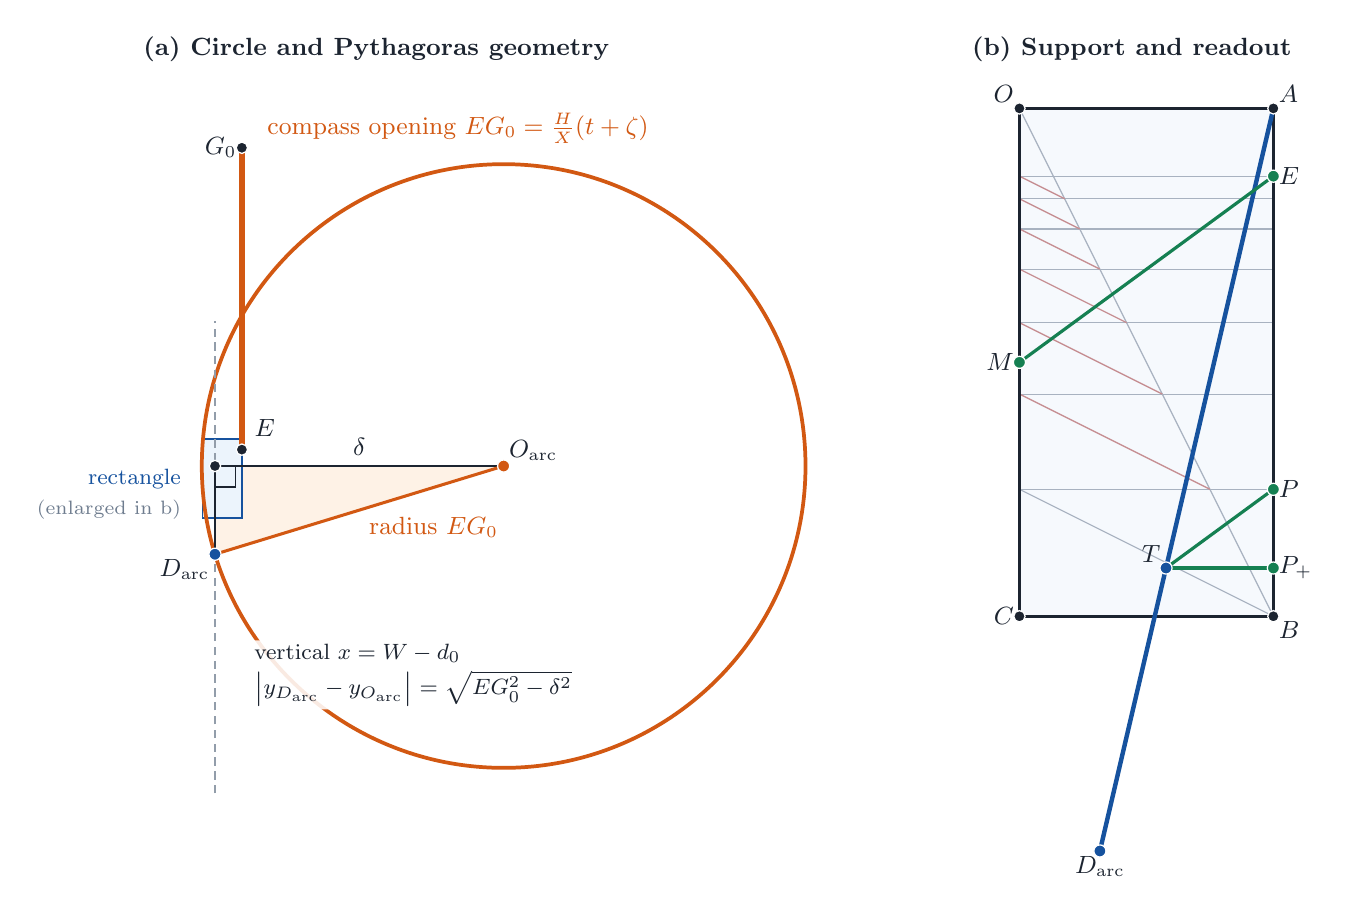
\begin{tikzpicture}[scale=0.25]
\node[ttl] at (-3.5,23.8) {(a) Circle and Pythagoras geometry};
\fill[trifill] (0.6337,-1.8484)--(0.6337,2.6337)--(15.2980,2.6337)--cycle;
\fill[bluefill] (0,0) rectangle (2.0,4.0);
\draw[line width=0.65pt,supp] (0,0) rectangle (2.0,4.0);
\draw[accent] (15.2980,2.6337) circle (15.3339);
\draw[aux] (0.6337,-14.0)--(0.6337,10.0);
\draw[accent,line width=2.4pt] (2.0000,3.4661)--(2.0000,18.8000);
\draw[line width=0.95pt,ink] (0.6337,-1.8484)--(0.6337,2.6337)--(15.2980,2.6337);
\draw[line width=1.1pt,acc] (15.2980,2.6337)--(0.6337,-1.8484);
\draw[line width=0.6pt,ink] (0.6337,1.5837)-|(1.6837,2.6337);
\node[pt] at (2.0000,18.8000) {};
\node[pt] at (2.0000,3.4661) {};
\node[pt] at (0.6337,2.6337) {};
\node[ptacc] at (15.2980,2.6337) {};
\node[ptsupp] at (0.6337,-1.8484) {};
\node[lab,left] at (2.0000,18.8000) {$G_0$};
\node[lab,halo,anchor=south west] at (2.4500,3.9161) {$E$};
\node[lab,above right] at (15.2980,2.6337) {$O_{\mathrm{arc}}$};
\node[lab,below left] at (0.6337,-1.8484) {$D_{\mathrm{arc}}$};
\node[lab,halo,text=acc,anchor=west] at (3.1000,19.8) {compass opening $EG_0=\frac HX(t+\zeta)$};
\node[lab,halo,above] at (7.9659,2.9837) {$\delta$};
\node[lab,halo,text=acc,anchor=north west] at (8.2659,0.2427) {radius $EG_0$};
\node[labsm,halo,anchor=north west,align=left] at (2.4337,-6.2) {vertical $x=W-d_0$\\[2pt]$\bigl|y_{D_{\mathrm{arc}}}-y_{O_{\mathrm{arc}}}\bigr|=\sqrt{EG_0^{2}-\delta^{2}}$};
\node[font=\footnotesize,text=supp,anchor=east] at (-0.6,2.0) {rectangle};
\node[font=\scriptsize,text=slatec,anchor=east] at (-0.6,0.4) {(enlarged in b)};
\begin{scope}[shift={(41.5,-5.0)},scale=6.45]
\node[ttl] at (-0.45,4.4651) {(b) Support and readout};
\fill[rectbg] (0.0000,0.0000) rectangle (2.0000,4.0000);
\draw[chain] (0.0000,4.0000)--(2.0000,0.0000);
\draw[chain] (0.0000,1.0000)--(2.0000,0.0000);
\draw[chain] (0,1.0000)--(2.0,1.0000);
\draw[chain] (0,1.7500)--(2.0,1.7500);
\draw[chain] (0,2.3125)--(2.0,2.3125);
\draw[chain] (0,2.7344)--(2.0,2.7344);
\draw[chain] (0,3.0508)--(2.0,3.0508);
\draw[chain] (0,3.2881)--(2.0,3.2881);
\draw[chain] (0,3.4661)--(2.0,3.4661);
\draw[chainpar] (1.5000,1.0000)--(0.0000,1.7500);
\draw[chainpar] (1.1250,1.7500)--(0.0000,2.3125);
\draw[chainpar] (0.8438,2.3125)--(0.0000,2.7344);
\draw[chainpar] (0.6328,2.7344)--(0.0000,3.0508);
\draw[chainpar] (0.4746,3.0508)--(0.0000,3.2881);
\draw[chainpar] (0.3560,3.2881)--(0.0000,3.4661);
\draw[rect] (0.0000,0.0000) rectangle (2.0000,4.0000);
\draw[support] (2.0000,4.0000)--(0.6337,-1.8484);
\draw[transport] (0.0000,2.0000)--(2.0000,3.4661);
\draw[transport] (2.0000,1.0000)--(1.1543,0.3801);
\draw[transport,line width=1.65pt] (1.1543,0.3801)--(2.0000,0.3801);
\node[lab,above left] at (0.0000,4.0000) {$O$};
\node[lab,above right] at (2.0000,4.0000) {$A$};
\node[lab,left] at (0.0000,0.0000) {$C$};
\node[lab,below right] at (2.0000,0.0000) {$B$};
\node[pt] at (0.0000,4.0000) {};
\node[pt] at (2.0000,4.0000) {};
\node[pt] at (0.0000,0.0000) {};
\node[pt] at (2.0000,0.0000) {};
\node[pttrans] at (0.0000,2.0000) {};
\node[pttrans] at (2.0000,3.4661) {};
\node[pttrans] at (2.0000,1.0000) {};
\node[ptsupp] at (1.1543,0.3801) {};
\node[pttrans] at (2.0000,0.3801) {};
\node[lab,left] at (0.0000,2.0000) {$M$};
\node[lab,right] at (2.0000,3.4661) {$E$};
\node[lab,right] at (2.0000,1.0000) {$P$};
\node[lab,right] at (2.0000,0.3801) {$P_+$};
\node[lab,above left] at (1.1543,0.3801) {$T$};
\node[ptsupp] at (0.6337,-1.8484) {};
\node[lab,below] at (0.6337,-1.8484) {$D_{\mathrm{arc}}$};
\end{scope}
\end{tikzpicture}%
}

\newcommand{\figMeanSteps}{%
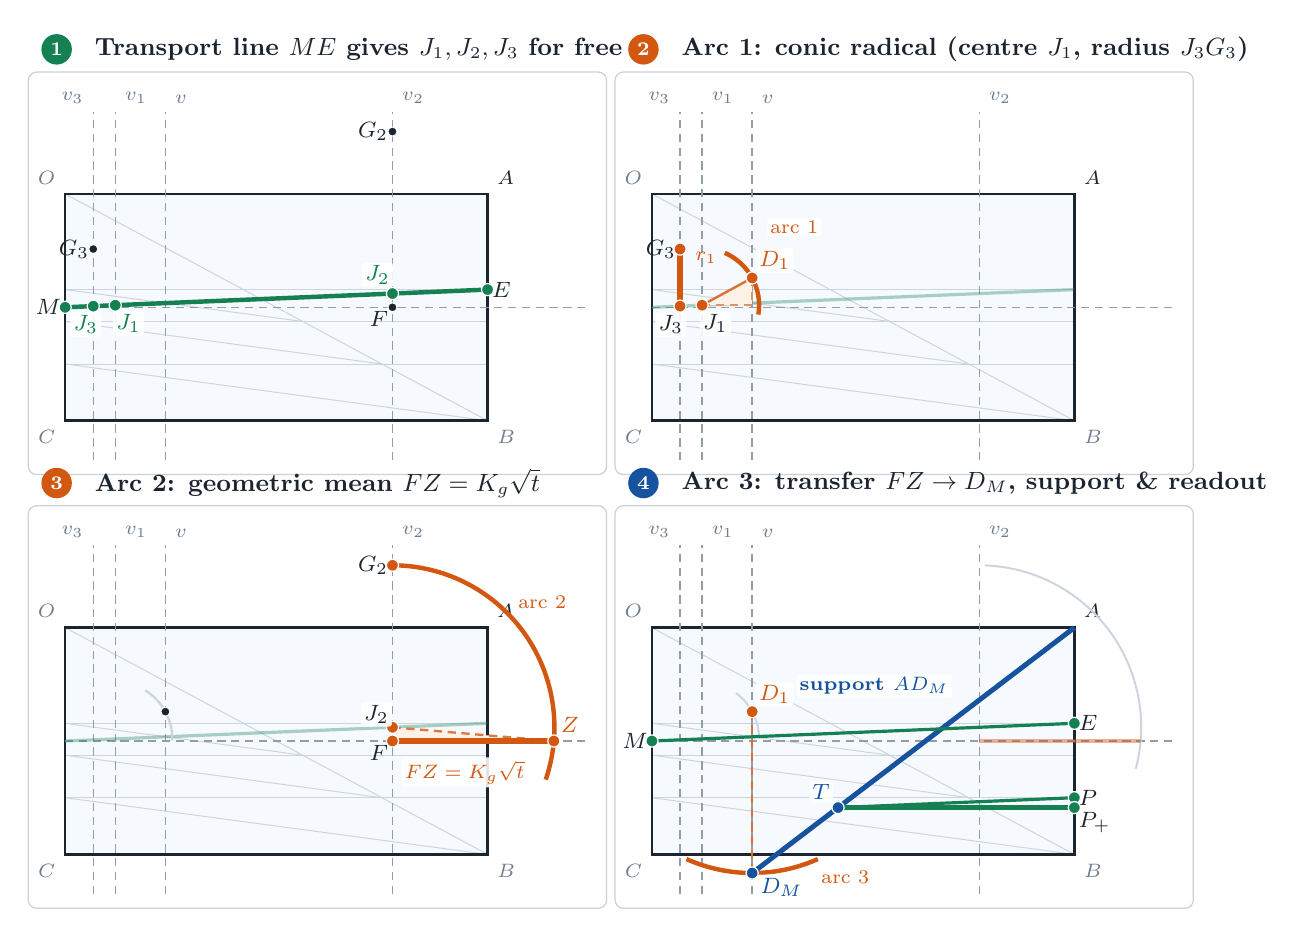
\begin{tikzpicture}[scale=0.72]
\begin{scope}[shift={(0,0)}]
\draw[line width=0.45pt,slatec!35,rounded corners=3pt,fill=white] (-0.65,-0.95) rectangle (9.55,6.15);
\fill[rectbg] (0.0000,0.0000) rectangle (7.4512,4.0000);
\draw[chainfaint] (0.0000,4.0000)--(7.4512,0.0000);
\draw[chainfaint] (0.0000,1.0000)--(7.4512,0.0000);
\draw[chainfaint] (0,1.0000)--(7.451155878422839,1.0000);
\draw[chainfaint] (0,1.7500)--(7.451155878422839,1.7500);
\draw[chainfaint] (0,2.3125)--(7.451155878422839,2.3125);
\draw[chainfaint] (5.5884,1.0000)--(0.0000,1.7500);
\draw[chainfaint] (4.1913,1.7500)--(0.0000,2.3125);
\draw[rect] (0.0000,0.0000) rectangle (7.4512,4.0000);
\draw[aux] (0.4961,-0.70)--(0.4961,5.45);
\draw[aux] (0.8840,-0.70)--(0.8840,5.45);
\draw[aux] (1.7681,-0.70)--(1.7681,5.45);
\draw[aux] (5.7733,-0.70)--(5.7733,5.45);
\draw[aux] (0,2.0000)--(9.20,2.0000);
\node[font=\scriptsize,text=slatec,anchor=south east] at (0.4961,5.42) {$v_3$};
\node[font=\scriptsize,text=slatec,anchor=south west] at (0.8840,5.42) {$v_1$};
\node[font=\scriptsize,text=slatec,anchor=south west] at (1.7681,5.42) {$v$};
\node[font=\scriptsize,text=slatec,anchor=south west] at (5.7733,5.42) {$v_2$};
\node[font=\scriptsize,text=slatec,above left] at (0.0000,4.0000) {$O$};
\node[font=\scriptsize,text=ink,above right] at (7.4512,4.0000) {$A$};
\node[font=\scriptsize,text=slatec,below left] at (0.0000,0.0000) {$C$};
\node[font=\scriptsize,text=slatec,below right] at (7.4512,0.0000) {$B$};
\node[badgetrans] at (-0.15,6.55) {1};
\node[ttl] at (0.35,6.55) {Transport line $ME$ gives $J_1, J_2, J_3$ for free};
\draw[transport,line width=1.6pt] (0.0000,2.0000)--(7.4512,2.3125);
\node[pttrans] at (0.0000,2.0000) {};
\node[pttrans] at (7.4512,2.3125) {};
\node[pttrans] at (0.8840,2.0371) {};
\node[pttrans] at (5.7733,2.2421) {};
\node[pttrans] at (0.4961,2.0208) {};
\node[ptsm] at (0.4961,3.0272) {};
\node[ptsm] at (5.7733,5.0993) {};
\node[ptsm] at (5.7733,2.0000) {};
\node[labsm,left] at (0.0000,2.0000) {$M$};
\node[labsm,right] at (7.4512,2.3125) {$E$};
\node[labsm,halo,text=trans,below left] at (0.6461,1.9208) {$J_3$};
\node[labsm,halo,text=trans,below right] at (0.8340,1.9371) {$J_1$};
\node[labsm,halo,text=trans,above left] at (5.7933,2.3421) {$J_2$};
\node[labsm,left] at (0.4961,3.0272) {$G_3$};
\node[labsm,left] at (5.7733,5.0993) {$G_2$};
\node[labsm,below left] at (5.7733,2.0000) {$F$};
\end{scope}
\begin{scope}[shift={(10.35,0)}]
\draw[line width=0.45pt,slatec!35,rounded corners=3pt,fill=white] (-0.65,-0.95) rectangle (9.55,6.15);
\fill[rectbg] (0.0000,0.0000) rectangle (7.4512,4.0000);
\draw[chainfaint] (0.0000,4.0000)--(7.4512,0.0000);
\draw[chainfaint] (0.0000,1.0000)--(7.4512,0.0000);
\draw[chainfaint] (0,1.0000)--(7.451155878422839,1.0000);
\draw[chainfaint] (0,1.7500)--(7.451155878422839,1.7500);
\draw[chainfaint] (0,2.3125)--(7.451155878422839,2.3125);
\draw[chainfaint] (5.5884,1.0000)--(0.0000,1.7500);
\draw[chainfaint] (4.1913,1.7500)--(0.0000,2.3125);
\draw[rect] (0.0000,0.0000) rectangle (7.4512,4.0000);
\draw[aux] (0.4961,-0.70)--(0.4961,5.45);
\draw[aux] (0.8840,-0.70)--(0.8840,5.45);
\draw[aux] (1.7681,-0.70)--(1.7681,5.45);
\draw[aux] (5.7733,-0.70)--(5.7733,5.45);
\draw[aux] (0,2.0000)--(9.20,2.0000);
\node[font=\scriptsize,text=slatec,anchor=south east] at (0.4961,5.42) {$v_3$};
\node[font=\scriptsize,text=slatec,anchor=south west] at (0.8840,5.42) {$v_1$};
\node[font=\scriptsize,text=slatec,anchor=south west] at (1.7681,5.42) {$v$};
\node[font=\scriptsize,text=slatec,anchor=south west] at (5.7733,5.42) {$v_2$};
\node[font=\scriptsize,text=slatec,above left] at (0.0000,4.0000) {$O$};
\node[font=\scriptsize,text=ink,above right] at (7.4512,4.0000) {$A$};
\node[font=\scriptsize,text=slatec,below left] at (0.0000,0.0000) {$C$};
\node[font=\scriptsize,text=slatec,below right] at (7.4512,0.0000) {$B$};
\node[badgeacc] at (-0.15,6.55) {2};
\node[ttl] at (0.35,6.55) {Arc 1: conic radical (centre $J_1$, radius $J_3G_3$)};
\draw[transport,opacity=0.35] (0.0000,2.0000)--(7.4512,2.3125);
\fill[trifill] (0.8840,2.0371)--(1.7681,2.0371)--(1.7681,2.5179)--cycle;
\draw[line width=0.65pt,acc!65,densely dashed] (0.8840,2.0371)--(1.7681,2.0371)--(1.7681,2.5179);
\draw[line width=0.85pt,acc!85] (0.8840,2.0371)--(1.7681,2.5179);
\draw[accent,line width=2.4pt] (0.4961,2.0208)--(0.4961,3.0272);
\draw[accent,line width=1.6pt] (0.8840,2.0371) ++(-9.46:1.0064) arc (-9.46:66.54:1.0064);
\node[ptacc] at (0.4961,2.0208) {};
\node[ptacc] at (0.4961,3.0272) {};
\node[ptacc] at (0.8840,2.0371) {};
\node[ptacc] at (1.7681,2.5179) {};
\node[labsm,left] at (0.4961,3.0272) {$G_3$};
\node[labsm,halo,below left] at (0.6161,1.9208) {$J_3$};
\node[labsm,halo,below right] at (0.8340,1.9371) {$J_1$};
\node[labsm,halo,text=acc,above right] at (1.8281,2.5979) {$D_1$};
\node[font=\scriptsize,halo,text=acc,anchor=west] at (2.0181,3.4179) {arc 1};
\node[font=\scriptsize,text=acc,anchor=west] at (0.5961,2.8740) {$r_1$};
\end{scope}
\begin{scope}[shift={(0,-7.65)}]
\draw[line width=0.45pt,slatec!35,rounded corners=3pt,fill=white] (-0.65,-0.95) rectangle (9.55,6.15);
\fill[rectbg] (0.0000,0.0000) rectangle (7.4512,4.0000);
\draw[chainfaint] (0.0000,4.0000)--(7.4512,0.0000);
\draw[chainfaint] (0.0000,1.0000)--(7.4512,0.0000);
\draw[chainfaint] (0,1.0000)--(7.451155878422839,1.0000);
\draw[chainfaint] (0,1.7500)--(7.451155878422839,1.7500);
\draw[chainfaint] (0,2.3125)--(7.451155878422839,2.3125);
\draw[chainfaint] (5.5884,1.0000)--(0.0000,1.7500);
\draw[chainfaint] (4.1913,1.7500)--(0.0000,2.3125);
\draw[rect] (0.0000,0.0000) rectangle (7.4512,4.0000);
\draw[aux] (0.4961,-0.70)--(0.4961,5.45);
\draw[aux] (0.8840,-0.70)--(0.8840,5.45);
\draw[aux] (1.7681,-0.70)--(1.7681,5.45);
\draw[aux] (5.7733,-0.70)--(5.7733,5.45);
\draw[aux] (0,2.0000)--(9.20,2.0000);
\node[font=\scriptsize,text=slatec,anchor=south east] at (0.4961,5.42) {$v_3$};
\node[font=\scriptsize,text=slatec,anchor=south west] at (0.8840,5.42) {$v_1$};
\node[font=\scriptsize,text=slatec,anchor=south west] at (1.7681,5.42) {$v$};
\node[font=\scriptsize,text=slatec,anchor=south west] at (5.7733,5.42) {$v_2$};
\node[font=\scriptsize,text=slatec,above left] at (0.0000,4.0000) {$O$};
\node[font=\scriptsize,text=ink,above right] at (7.4512,4.0000) {$A$};
\node[font=\scriptsize,text=slatec,below left] at (0.0000,0.0000) {$C$};
\node[font=\scriptsize,text=slatec,below right] at (7.4512,0.0000) {$B$};
\node[badgeacc] at (-0.15,6.55) {3};
\node[ttl] at (0.35,6.55) {Arc 2: geometric mean $FZ = K_g\sqrt{t}$};
\draw[transport,opacity=0.35] (0.0000,2.0000)--(7.4512,2.3125);
\draw[faint,line width=0.8pt] (0.8840,2.0371) ++(-1.46:1.0064) arc (-1.46:58.54:1.0064);
\fill[trifill] (5.7733,2.0000)--(5.7733,2.2421)--(8.6202,2.0000)--cycle;
\draw[line width=0.85pt,acc!80,densely dashed] (5.7733,2.2421)--(8.6202,2.0000);
\draw[accent,line width=2.4pt] (5.7733,2.0000)--(8.6202,2.0000);
\draw[accent,line width=1.6pt] (5.7733,2.2421) ++(-18.86:2.8571) arc (-18.86:90.00:2.8571);
\node[ptacc] at (5.7733,2.2421) {};
\node[ptacc] at (5.7733,5.0993) {};
\node[ptacc] at (5.7733,2.0000) {};
\node[ptacc] at (8.6202,2.0000) {};
\node[ptsm] at (1.7681,2.5179) {};
\node[labsm,left] at (5.7733,5.0993) {$G_2$};
\node[labsm,halo,above left] at (5.7733,2.2421) {$J_2$};
\node[labsm,below left] at (5.7733,2.0000) {$F$};
\node[labsm,halo,text=acc,above right] at (8.6802,2.0800) {$Z$};
\node[font=\scriptsize,halo,text=acc,anchor=north] at (7.0467,1.7200) {$FZ = K_g\sqrt{t}$};
\node[font=\scriptsize,halo,text=acc,anchor=west] at (7.9233,4.45) {arc 2};
\end{scope}
\begin{scope}[shift={(10.35,-7.65)}]
\draw[line width=0.45pt,slatec!35,rounded corners=3pt,fill=white] (-0.65,-0.95) rectangle (9.55,6.15);
\fill[rectbg] (0.0000,0.0000) rectangle (7.4512,4.0000);
\draw[chainfaint] (0.0000,4.0000)--(7.4512,0.0000);
\draw[chainfaint] (0.0000,1.0000)--(7.4512,0.0000);
\draw[chainfaint] (0,1.0000)--(7.451155878422839,1.0000);
\draw[chainfaint] (0,1.7500)--(7.451155878422839,1.7500);
\draw[chainfaint] (0,2.3125)--(7.451155878422839,2.3125);
\draw[chainfaint] (5.5884,1.0000)--(0.0000,1.7500);
\draw[chainfaint] (4.1913,1.7500)--(0.0000,2.3125);
\draw[rect] (0.0000,0.0000) rectangle (7.4512,4.0000);
\draw[aux] (0.4961,-0.70)--(0.4961,5.45);
\draw[aux] (0.8840,-0.70)--(0.8840,5.45);
\draw[aux] (1.7681,-0.70)--(1.7681,5.45);
\draw[aux] (5.7733,-0.70)--(5.7733,5.45);
\draw[aux] (0,2.0000)--(9.20,2.0000);
\node[font=\scriptsize,text=slatec,anchor=south east] at (0.4961,5.42) {$v_3$};
\node[font=\scriptsize,text=slatec,anchor=south west] at (0.8840,5.42) {$v_1$};
\node[font=\scriptsize,text=slatec,anchor=south west] at (1.7681,5.42) {$v$};
\node[font=\scriptsize,text=slatec,anchor=south west] at (5.7733,5.42) {$v_2$};
\node[font=\scriptsize,text=slatec,above left] at (0.0000,4.0000) {$O$};
\node[font=\scriptsize,text=ink,above right] at (7.4512,4.0000) {$A$};
\node[font=\scriptsize,text=slatec,below left] at (0.0000,0.0000) {$C$};
\node[font=\scriptsize,text=slatec,below right] at (7.4512,0.0000) {$B$};
\node[badge] at (-0.15,6.55) {4};
\node[ttl] at (0.35,6.55) {Arc 3: transfer $FZ \to D_M$, support \& readout};
\draw[faint,line width=0.7pt] (0.8840,2.0371) ++(3.54:1.0064) arc (3.54:53.54:1.0064);
\draw[faint,line width=0.7pt] (5.7733,2.2421) ++(-14.86:2.8571) arc (-14.86:88.00:2.8571);
\draw[accent,opacity=0.45,line width=1.6pt] (5.7733,2.0000)--(8.6202,2.0000);
\draw[line width=0.85pt,acc!85,densely dashed] (1.7681,2.5179)--(1.7681,-0.3289);
\draw[accent,line width=1.6pt] (1.7681,2.5179) ++(-114.00:2.8469) arc (-114.00:-66.00:2.8469);
\draw[support,line width=1.8pt] (7.4512,4.0000)--(1.7681,-0.3289);
\draw[transport] (0.0000,2.0000)--(7.4512,2.3125);
\draw[transport] (7.4512,1.0000)--(3.2832,0.8252);
\draw[transport,line width=1.65pt] (3.2832,0.8252)--(7.4512,0.8252);
\node[pttrans] at (0.0000,2.0000) {};
\node[pttrans] at (7.4512,2.3125) {};
\node[pttrans] at (7.4512,1.0000) {};
\node[pttrans] at (7.4512,0.8252) {};
\node[ptacc] at (1.7681,2.5179) {};
\node[ptsupp] at (1.7681,-0.3289) {};
\node[ptsupp] at (3.2832,0.8252) {};
\node[labsm,left] at (0.0000,2.0000) {$M$};
\node[labsm,right] at (7.4512,2.3125) {$E$};
\node[labsm,right] at (7.4512,1.0000) {$P$};
\node[labsm,below right] at (7.4512,0.8252) {$P_+$};
\node[labsm,halo,text=supp,above left] at (3.2032,0.9052) {$T$};
\node[labsm,halo,text=acc,above right] at (1.8281,2.5979) {$D_1$};
\node[labsm,halo,text=supp,below right] at (1.8481,-0.3489) {$D_M$};
\node[font=\scriptsize,halo,text=acc,anchor=west] at (2.9181,-0.4089) {arc 3};
\node[font=\scriptsize\bfseries,halo,text=supp,anchor=south east] at (5.30,2.75) {support $AD_M$};
\end{scope}
\end{tikzpicture}%
}

\newcommand{\figEfficiency}{%
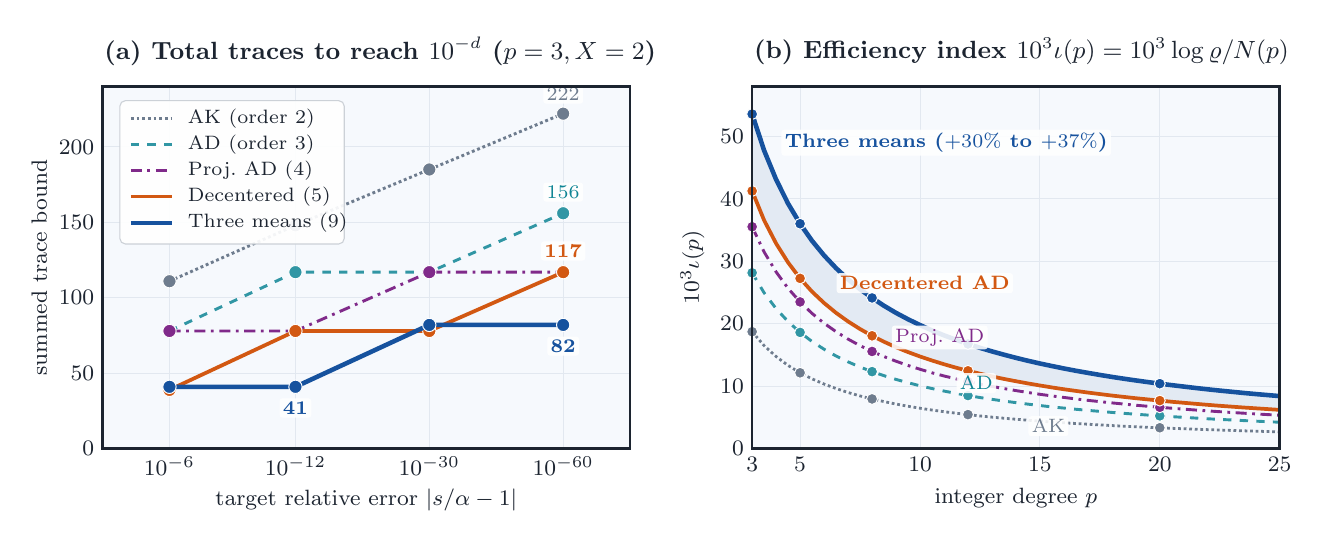
\begin{tikzpicture}
\begin{scope}[shift={(0,0)}]
\node[ttl] at (-0.1,5.050) {(a) Total traces to reach $10^{-d}$ ($p=3, X=2$)};
\fill[rectbg] (0,0) rectangle (6.700,4.600);
\draw[line width=0.35pt,gridc] (0,0.000)--(6.700,0.000);
\node[labsm,left] at (-0.05,0.000) {0};
\draw[line width=0.35pt,gridc] (0,0.958)--(6.700,0.958);
\node[labsm,left] at (-0.05,0.958) {50};
\draw[line width=0.35pt,gridc] (0,1.917)--(6.700,1.917);
\node[labsm,left] at (-0.05,1.917) {100};
\draw[line width=0.35pt,gridc] (0,2.875)--(6.700,2.875);
\node[labsm,left] at (-0.05,2.875) {150};
\draw[line width=0.35pt,gridc] (0,3.833)--(6.700,3.833);
\node[labsm,left] at (-0.05,3.833) {200};
\draw[line width=0.35pt,gridc] (0.850,0)--(0.850,4.600);
\node[labsm,below] at (0.850,-0.05) {$10^{-6}$};
\draw[line width=0.35pt,gridc] (2.450,0)--(2.450,4.600);
\node[labsm,below] at (2.450,-0.05) {$10^{-12}$};
\draw[line width=0.35pt,gridc] (4.150,0)--(4.150,4.600);
\node[labsm,below] at (4.150,-0.05) {$10^{-30}$};
\draw[line width=0.35pt,gridc] (5.850,0)--(5.850,4.600);
\node[labsm,below] at (5.850,-0.05) {$10^{-60}$};
\draw[slatec,densely dotted,line width=1.05pt] (0.850,2.127)--(2.450,2.837)--(4.150,3.546)--(5.850,4.255);
\node[circle,fill=slatec,draw=white,line width=0.35pt,inner sep=1.7pt] at (0.850,2.127) {};
\node[circle,fill=slatec,draw=white,line width=0.35pt,inner sep=1.7pt] at (2.450,2.837) {};
\node[circle,fill=slatec,draw=white,line width=0.35pt,inner sep=1.7pt] at (4.150,3.546) {};
\node[circle,fill=slatec,draw=white,line width=0.35pt,inner sep=1.7pt] at (5.850,4.255) {};
\draw[tealc!85,dashed,line width=1.05pt] (0.850,1.495)--(2.450,2.242)--(4.150,2.242)--(5.850,2.990);
\node[circle,fill=tealc!85,draw=white,line width=0.35pt,inner sep=1.7pt] at (0.850,1.495) {};
\node[circle,fill=tealc!85,draw=white,line width=0.35pt,inner sep=1.7pt] at (2.450,2.242) {};
\node[circle,fill=tealc!85,draw=white,line width=0.35pt,inner sep=1.7pt] at (4.150,2.242) {};
\node[circle,fill=tealc!85,draw=white,line width=0.35pt,inner sep=1.7pt] at (5.850,2.990) {};
\draw[plum,dash pattern=on 4pt off 2pt on 1pt off 2pt,line width=1.05pt] (0.850,1.495)--(2.450,1.495)--(4.150,2.242)--(5.850,2.242);
\node[circle,fill=plum,draw=white,line width=0.35pt,inner sep=1.7pt] at (0.850,1.495) {};
\node[circle,fill=plum,draw=white,line width=0.35pt,inner sep=1.7pt] at (2.450,1.495) {};
\node[circle,fill=plum,draw=white,line width=0.35pt,inner sep=1.7pt] at (4.150,2.242) {};
\node[circle,fill=plum,draw=white,line width=0.35pt,inner sep=1.7pt] at (5.850,2.242) {};
\draw[acc,solid,line width=1.35pt] (0.850,0.747)--(2.450,1.495)--(4.150,1.495)--(5.850,2.242);
\node[circle,fill=acc,draw=white,line width=0.35pt,inner sep=1.7pt] at (0.850,0.747) {};
\node[circle,fill=acc,draw=white,line width=0.35pt,inner sep=1.7pt] at (2.450,1.495) {};
\node[circle,fill=acc,draw=white,line width=0.35pt,inner sep=1.7pt] at (4.150,1.495) {};
\node[circle,fill=acc,draw=white,line width=0.35pt,inner sep=1.7pt] at (5.850,2.242) {};
\draw[supp,solid,line width=1.65pt] (0.850,0.786)--(2.450,0.786)--(4.150,1.572)--(5.850,1.572);
\node[circle,fill=supp,draw=white,line width=0.35pt,inner sep=1.7pt] at (0.850,0.786) {};
\node[circle,fill=supp,draw=white,line width=0.35pt,inner sep=1.7pt] at (2.450,0.786) {};
\node[circle,fill=supp,draw=white,line width=0.35pt,inner sep=1.7pt] at (4.150,1.572) {};
\node[circle,fill=supp,draw=white,line width=0.35pt,inner sep=1.7pt] at (5.850,1.572) {};
\node[font=\scriptsize\bfseries,text=supp,halo,anchor=north] at (5.850,1.432) {82};
\node[font=\scriptsize\bfseries,text=acc,halo,anchor=south] at (5.850,2.382) {117};
\node[font=\scriptsize,text=tealc,halo,anchor=south] at (5.850,3.130) {156};
\node[font=\scriptsize,text=slatec,halo,anchor=south] at (5.850,4.375) {222};
\node[font=\scriptsize\bfseries,text=supp,halo,anchor=north] at (2.450,0.646) {41};
\fill[white,fill opacity=0.92,draw=slatec!35,rounded corners=2pt] (0.22,2.60) rectangle (3.07,4.42);
\draw[slatec,densely dotted,line width=1.05pt] (0.36,4.19)--(0.88,4.19);
\node[font=\scriptsize,text=ink,anchor=west] at (0.96,4.19) {AK (order 2)};
\draw[tealc!85,dashed,line width=1.05pt] (0.36,3.86)--(0.88,3.86);
\node[font=\scriptsize,text=ink,anchor=west] at (0.96,3.86) {AD (order 3)};
\draw[plum,dash pattern=on 4pt off 2pt on 1pt off 2pt,line width=1.05pt] (0.36,3.53)--(0.88,3.53);
\node[font=\scriptsize,text=ink,anchor=west] at (0.96,3.53) {Proj.\ AD (4)};
\draw[acc,solid,line width=1.05pt] (0.36,3.20)--(0.88,3.20);
\node[font=\scriptsize,text=ink,anchor=west] at (0.96,3.20) {Decentered (5)};
\draw[supp,solid,line width=1.5pt] (0.36,2.87)--(0.88,2.87);
\node[font=\scriptsize,text=ink,anchor=west] at (0.96,2.87) {Three means (9)};
\draw[rect] (0,0) rectangle (6.700,4.600);
\node[labsm,anchor=north] at (3.350,-0.45) {target relative error $|s/\alpha-1|$};
\node[labsm,rotate=90,anchor=south] at (-0.65,2.300) {summed trace bound};
\end{scope}
\begin{scope}[shift={(8.250,0)}]
\node[ttl] at (-0.1,5.050) {(b) Efficiency index $10^3\iota(p)=10^3\log\varrho/N(p)$};
\fill[rectbg] (0,0) rectangle (6.700,4.600);
\draw[line width=0.35pt,gridc] (0.000,0)--(0.000,4.600);
\node[labsm,below] at (0.000,-0.05) {3};
\draw[line width=0.35pt,gridc] (0.609,0)--(0.609,4.600);
\node[labsm,below] at (0.609,-0.05) {5};
\draw[line width=0.35pt,gridc] (2.132,0)--(2.132,4.600);
\node[labsm,below] at (2.132,-0.05) {10};
\draw[line width=0.35pt,gridc] (3.655,0)--(3.655,4.600);
\node[labsm,below] at (3.655,-0.05) {15};
\draw[line width=0.35pt,gridc] (5.177,0)--(5.177,4.600);
\node[labsm,below] at (5.177,-0.05) {20};
\draw[line width=0.35pt,gridc] (6.700,0)--(6.700,4.600);
\node[labsm,below] at (6.700,-0.05) {25};
\draw[line width=0.35pt,gridc] (0,0.000)--(6.700,0.000);
\node[labsm,left] at (-0.05,0.000) {0};
\draw[line width=0.35pt,gridc] (0,0.793)--(6.700,0.793);
\node[labsm,left] at (-0.05,0.793) {10};
\draw[line width=0.35pt,gridc] (0,1.586)--(6.700,1.586);
\node[labsm,left] at (-0.05,1.586) {20};
\draw[line width=0.35pt,gridc] (0,2.379)--(6.700,2.379);
\node[labsm,left] at (-0.05,2.379) {30};
\draw[line width=0.35pt,gridc] (0,3.172)--(6.700,3.172);
\node[labsm,left] at (-0.05,3.172) {40};
\draw[line width=0.35pt,gridc] (0,3.966)--(6.700,3.966);
\node[labsm,left] at (-0.05,3.966) {50};
\fill[supp!12] (0.000,4.250)--(0.152,3.788)--(0.305,3.417)--(0.457,3.112)--(0.609,2.857)--(0.761,2.640)--(0.914,2.454)--(1.066,2.293)--(1.218,2.151)--(1.370,2.026)--(1.523,1.915)--(1.675,1.815)--(1.827,1.725)--(1.980,1.644)--(2.132,1.570)--(2.284,1.502)--(2.436,1.440)--(2.589,1.383)--(2.741,1.330)--(2.893,1.281)--(3.045,1.236)--(3.198,1.194)--(3.350,1.154)--(3.502,1.117)--(3.655,1.082)--(3.807,1.050)--(3.959,1.019)--(4.111,0.990)--(4.264,0.963)--(4.416,0.937)--(4.568,0.912)--(4.720,0.889)--(4.873,0.867)--(5.025,0.846)--(5.177,0.826)--(5.330,0.807)--(5.482,0.789)--(5.634,0.771)--(5.786,0.754)--(5.939,0.738)--(6.091,0.723)--(6.243,0.708)--(6.395,0.694)--(6.548,0.681)--(6.700,0.668)--(6.700,0.493)--(6.548,0.503)--(6.395,0.513)--(6.243,0.523)--(6.091,0.534)--(5.939,0.545)--(5.786,0.557)--(5.634,0.570)--(5.482,0.583)--(5.330,0.596)--(5.177,0.611)--(5.025,0.626)--(4.873,0.641)--(4.720,0.658)--(4.568,0.675)--(4.416,0.694)--(4.264,0.713)--(4.111,0.734)--(3.959,0.755)--(3.807,0.778)--(3.655,0.803)--(3.502,0.829)--(3.350,0.857)--(3.198,0.886)--(3.045,0.918)--(2.893,0.953)--(2.741,0.989)--(2.589,1.029)--(2.436,1.073)--(2.284,1.120)--(2.132,1.171)--(1.980,1.227)--(1.827,1.289)--(1.675,1.358)--(1.523,1.434)--(1.370,1.520)--(1.218,1.616)--(1.066,1.725)--(0.914,1.850)--(0.761,1.994)--(0.609,2.163)--(0.457,2.364)--(0.305,2.605)--(0.152,2.901)--(0.000,3.273)--cycle;
\draw[slatec,densely dotted,line width=1.0pt] (0.000,1.486)--(0.152,1.309)--(0.305,1.170)--(0.457,1.057)--(0.609,0.964)--(0.761,0.887)--(0.914,0.821)--(1.066,0.764)--(1.218,0.714)--(1.370,0.670)--(1.523,0.632)--(1.675,0.598)--(1.827,0.567)--(1.980,0.539)--(2.132,0.514)--(2.284,0.491)--(2.436,0.470)--(2.589,0.451)--(2.741,0.433)--(2.893,0.416)--(3.045,0.401)--(3.198,0.387)--(3.350,0.374)--(3.502,0.362)--(3.655,0.350)--(3.807,0.339)--(3.959,0.329)--(4.111,0.320)--(4.264,0.311)--(4.416,0.302)--(4.568,0.294)--(4.720,0.286)--(4.873,0.279)--(5.025,0.272)--(5.177,0.266)--(5.330,0.259)--(5.482,0.253)--(5.634,0.248)--(5.786,0.242)--(5.939,0.237)--(6.091,0.232)--(6.243,0.227)--(6.395,0.223)--(6.548,0.218)--(6.700,0.214);
\node[circle,fill=slatec,draw=white,line width=0.35pt,inner sep=1.4pt] at (0.000,1.486) {};
\node[circle,fill=slatec,draw=white,line width=0.35pt,inner sep=1.4pt] at (0.609,0.964) {};
\node[circle,fill=slatec,draw=white,line width=0.35pt,inner sep=1.4pt] at (1.523,0.632) {};
\node[circle,fill=slatec,draw=white,line width=0.35pt,inner sep=1.4pt] at (2.741,0.433) {};
\node[circle,fill=slatec,draw=white,line width=0.35pt,inner sep=1.4pt] at (5.177,0.266) {};
\draw[tealc!85,dashed,line width=1.05pt] (0.000,2.234)--(0.152,1.980)--(0.305,1.778)--(0.457,1.614)--(0.609,1.477)--(0.761,1.361)--(0.914,1.263)--(1.066,1.177)--(1.218,1.103)--(1.370,1.037)--(1.523,0.979)--(1.675,0.927)--(1.827,0.880)--(1.980,0.838)--(2.132,0.799)--(2.284,0.764)--(2.436,0.732)--(2.589,0.703)--(2.741,0.675)--(2.893,0.650)--(3.045,0.627)--(3.198,0.605)--(3.350,0.585)--(3.502,0.566)--(3.655,0.548)--(3.807,0.531)--(3.959,0.516)--(4.111,0.501)--(4.264,0.487)--(4.416,0.474)--(4.568,0.461)--(4.720,0.449)--(4.873,0.438)--(5.025,0.427)--(5.177,0.417)--(5.330,0.407)--(5.482,0.398)--(5.634,0.389)--(5.786,0.380)--(5.939,0.372)--(6.091,0.365)--(6.243,0.357)--(6.395,0.350)--(6.548,0.343)--(6.700,0.336);
\node[circle,fill=tealc!85,draw=white,line width=0.35pt,inner sep=1.4pt] at (0.000,2.234) {};
\node[circle,fill=tealc!85,draw=white,line width=0.35pt,inner sep=1.4pt] at (0.609,1.477) {};
\node[circle,fill=tealc!85,draw=white,line width=0.35pt,inner sep=1.4pt] at (1.523,0.979) {};
\node[circle,fill=tealc!85,draw=white,line width=0.35pt,inner sep=1.4pt] at (2.741,0.675) {};
\node[circle,fill=tealc!85,draw=white,line width=0.35pt,inner sep=1.4pt] at (5.177,0.417) {};
\draw[plum,dash pattern=on 4pt off 2pt on 1pt off 2pt,line width=1.05pt] (0.000,2.819)--(0.152,2.499)--(0.305,2.244)--(0.457,2.036)--(0.609,1.864)--(0.761,1.718)--(0.914,1.593)--(1.066,1.486)--(1.218,1.392)--(1.370,1.309)--(1.523,1.235)--(1.675,1.170)--(1.827,1.111)--(1.980,1.057)--(2.132,1.009)--(2.284,0.964)--(2.436,0.924)--(2.589,0.887)--(2.741,0.852)--(2.893,0.821)--(3.045,0.791)--(3.198,0.764)--(3.350,0.738)--(3.502,0.714)--(3.655,0.691)--(3.807,0.670)--(3.959,0.651)--(4.111,0.632)--(4.264,0.614)--(4.416,0.598)--(4.568,0.582)--(4.720,0.567)--(4.873,0.552)--(5.025,0.539)--(5.177,0.526)--(5.330,0.514)--(5.482,0.502)--(5.634,0.491)--(5.786,0.480)--(5.939,0.470)--(6.091,0.460)--(6.243,0.451)--(6.395,0.442)--(6.548,0.433)--(6.700,0.425);
\node[circle,fill=plum,draw=white,line width=0.35pt,inner sep=1.4pt] at (0.000,2.819) {};
\node[circle,fill=plum,draw=white,line width=0.35pt,inner sep=1.4pt] at (0.609,1.864) {};
\node[circle,fill=plum,draw=white,line width=0.35pt,inner sep=1.4pt] at (1.523,1.235) {};
\node[circle,fill=plum,draw=white,line width=0.35pt,inner sep=1.4pt] at (2.741,0.852) {};
\node[circle,fill=plum,draw=white,line width=0.35pt,inner sep=1.4pt] at (5.177,0.526) {};
\draw[acc,solid,line width=1.35pt] (0.000,3.273)--(0.152,2.901)--(0.305,2.605)--(0.457,2.364)--(0.609,2.163)--(0.761,1.994)--(0.914,1.850)--(1.066,1.725)--(1.218,1.616)--(1.370,1.520)--(1.523,1.434)--(1.675,1.358)--(1.827,1.289)--(1.980,1.227)--(2.132,1.171)--(2.284,1.120)--(2.436,1.073)--(2.589,1.029)--(2.741,0.989)--(2.893,0.953)--(3.045,0.918)--(3.198,0.886)--(3.350,0.857)--(3.502,0.829)--(3.655,0.803)--(3.807,0.778)--(3.959,0.755)--(4.111,0.734)--(4.264,0.713)--(4.416,0.694)--(4.568,0.675)--(4.720,0.658)--(4.873,0.641)--(5.025,0.626)--(5.177,0.611)--(5.330,0.596)--(5.482,0.583)--(5.634,0.570)--(5.786,0.557)--(5.939,0.545)--(6.091,0.534)--(6.243,0.523)--(6.395,0.513)--(6.548,0.503)--(6.700,0.493);
\node[circle,fill=acc,draw=white,line width=0.35pt,inner sep=1.4pt] at (0.000,3.273) {};
\node[circle,fill=acc,draw=white,line width=0.35pt,inner sep=1.4pt] at (0.609,2.163) {};
\node[circle,fill=acc,draw=white,line width=0.35pt,inner sep=1.4pt] at (1.523,1.434) {};
\node[circle,fill=acc,draw=white,line width=0.35pt,inner sep=1.4pt] at (2.741,0.989) {};
\node[circle,fill=acc,draw=white,line width=0.35pt,inner sep=1.4pt] at (5.177,0.611) {};
\draw[supp,solid,line width=1.65pt] (0.000,4.250)--(0.152,3.788)--(0.305,3.417)--(0.457,3.112)--(0.609,2.857)--(0.761,2.640)--(0.914,2.454)--(1.066,2.293)--(1.218,2.151)--(1.370,2.026)--(1.523,1.915)--(1.675,1.815)--(1.827,1.725)--(1.980,1.644)--(2.132,1.570)--(2.284,1.502)--(2.436,1.440)--(2.589,1.383)--(2.741,1.330)--(2.893,1.281)--(3.045,1.236)--(3.198,1.194)--(3.350,1.154)--(3.502,1.117)--(3.655,1.082)--(3.807,1.050)--(3.959,1.019)--(4.111,0.990)--(4.264,0.963)--(4.416,0.937)--(4.568,0.912)--(4.720,0.889)--(4.873,0.867)--(5.025,0.846)--(5.177,0.826)--(5.330,0.807)--(5.482,0.789)--(5.634,0.771)--(5.786,0.754)--(5.939,0.738)--(6.091,0.723)--(6.243,0.708)--(6.395,0.694)--(6.548,0.681)--(6.700,0.668);
\node[circle,fill=supp,draw=white,line width=0.35pt,inner sep=1.4pt] at (0.000,4.250) {};
\node[circle,fill=supp,draw=white,line width=0.35pt,inner sep=1.4pt] at (0.609,2.857) {};
\node[circle,fill=supp,draw=white,line width=0.35pt,inner sep=1.4pt] at (1.523,1.915) {};
\node[circle,fill=supp,draw=white,line width=0.35pt,inner sep=1.4pt] at (2.741,1.330) {};
\node[circle,fill=supp,draw=white,line width=0.35pt,inner sep=1.4pt] at (5.177,0.826) {};
\node[font=\scriptsize\bfseries,text=supp,halo,anchor=west] at (0.365,3.886) {Three means ($+30\%$ to $+37\%$)};
\node[font=\scriptsize\bfseries,text=acc,halo,anchor=west] at (1.066,2.102) {Decentered AD};
\node[font=\scriptsize,text=plum,halo,anchor=west] at (1.766,1.412) {Proj.\ AD};
\node[font=\scriptsize,text=tealc,halo,anchor=west] at (2.589,0.833) {AD};
\node[font=\scriptsize,text=slatec,halo,anchor=west] at (3.502,0.286) {AK};
\draw[rect] (0,0) rectangle (6.700,4.600);
\node[labsm,anchor=north] at (3.350,-0.45) {integer degree $p$};
\node[labsm,rotate=90,anchor=south] at (-0.55,2.300) {$10^3\iota(p)$};
\end{scope}
\end{tikzpicture}%
}

\newcommand{\figSubdivision}{%
\begin{tikzpicture}[scale=2.15]
\fill[bluefill] (0,0)--(4.0,0) arc (0:180:2.0)--cycle;
\fill[trifill] (0,0)--(1.2,0)--(1.2,1.8330)--cycle;
\draw[line width=1.45pt,supp] (4.0,0) arc (0:180:2.0);
\draw[rect] (0,0)--(4.0,0);
\draw[line width=0.75pt,slatec] (0,0)--(1.2,1.8330)--(4.0,0);
\draw[accent,line width=2.2pt] (1.2,0)--(1.2,1.8330);
\draw[line width=0.55pt,ink] (1.3400,0)|-(1.2000,0.14);
\node[pt] at (0.0000,0.0000) {};
\node[pt] at (2.0000,0.0000) {};
\node[pt] at (4.0000,0.0000) {};
\node[ptacc] at (1.2,0) {};
\node[ptacc] at (1.2,1.8330) {};
\node[lab,below left] at (0,0) {$O$};
\node[lab,below] at (1.2,-0.03) {$T$};
\node[lab,below] at (2.0,-0.03) {$C$};
\node[lab,below right] at (4.0,0) {$S$};
\node[lab,above left] at (1.2,1.8330) {$G$};
\node[lab,halo,text=acc,anchor=west] at (1.28,0.8065) {$TG=m=\sqrt{ab}$};
\draw[dim] (0,-0.40)--(1.2,-0.40) node[midway,below,lab] {$a$};
\draw[dim] (1.2,-0.40)--(4.0,-0.40) node[midway,below,lab] {$b$};
\node[card,anchor=west,align=left,font=\small,inner sep=7pt] at (4.35,1.02) {\textbf{Subdivision update}\\[4pt]$\lambda\le\tfrac12:\quad (a,b,\lambda)\mapsto(a,\,m,\,2\lambda)$\\[4pt]$\lambda>\tfrac12:\quad (a,b,\lambda)\mapsto(m,\,b,\,2\lambda-1)$\\[5pt]\textcolor{supp}{\textbf{Gap:}}\quad $b/a\ \mapsto\ \sqrt{b/a}$};
\end{tikzpicture}%
}

\newcommand{\figDepth}{%
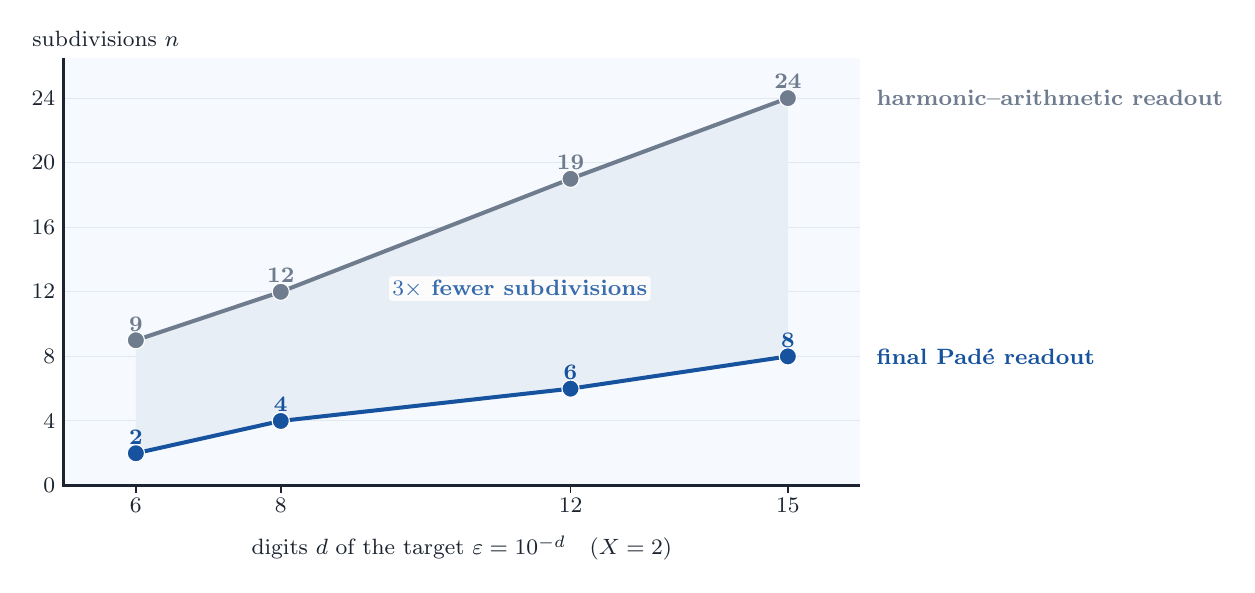
\begin{tikzpicture}
\fill[rectbg] (0,0) rectangle (10.120,5.433);
\draw[line width=0.35pt,gridc] (0,0.000)--(10.120,0.000);
\node[labsm,left] at (-0.05,0.000) {0};
\draw[line width=0.35pt,gridc] (0,0.820)--(10.120,0.820);
\node[labsm,left] at (-0.05,0.820) {4};
\draw[line width=0.35pt,gridc] (0,1.640)--(10.120,1.640);
\node[labsm,left] at (-0.05,1.640) {8};
\draw[line width=0.35pt,gridc] (0,2.460)--(10.120,2.460);
\node[labsm,left] at (-0.05,2.460) {12};
\draw[line width=0.35pt,gridc] (0,3.280)--(10.120,3.280);
\node[labsm,left] at (-0.05,3.280) {16};
\draw[line width=0.35pt,gridc] (0,4.100)--(10.120,4.100);
\node[labsm,left] at (-0.05,4.100) {20};
\draw[line width=0.35pt,gridc] (0,4.920)--(10.120,4.920);
\node[labsm,left] at (-0.05,4.920) {24};
\fill[supp!10] (0.920,1.845)--(2.760,2.460)--(6.440,3.895)--(9.200,4.920)--(9.200,1.640)--(6.440,1.230)--(2.760,0.820)--(0.920,0.410)--cycle;
\node[font=\footnotesize\bfseries,text=supp!85,halo] at (5.796,2.501) {$3\times$ fewer subdivisions};
\draw[rect] (0,5.433)--(0,0)--(10.120,0);
\draw[line width=0.6pt,ink] (0.920,0)--(0.920,-0.1);
\node[labsm,below] at (0.920,-0.1) {6};
\draw[line width=0.6pt,ink] (2.760,0)--(2.760,-0.1);
\node[labsm,below] at (2.760,-0.1) {8};
\draw[line width=0.6pt,ink] (6.440,0)--(6.440,-0.1);
\node[labsm,below] at (6.440,-0.1) {12};
\draw[line width=0.6pt,ink] (9.200,0)--(9.200,-0.1);
\node[labsm,below] at (9.200,-0.1) {15};
\draw[line width=1.45pt,slatec] (0.920,1.845)--(2.760,2.460)--(6.440,3.895)--(9.200,4.920);
\node[circle,fill=slatec,draw=white,line width=0.4pt,inner sep=2.2pt] at (0.920,1.845) {};
\node[labsm,above,slatec] at (0.920,1.905) {\textbf{9}};
\node[circle,fill=slatec,draw=white,line width=0.4pt,inner sep=2.2pt] at (2.760,2.460) {};
\node[labsm,above,slatec] at (2.760,2.520) {\textbf{12}};
\node[circle,fill=slatec,draw=white,line width=0.4pt,inner sep=2.2pt] at (6.440,3.895) {};
\node[labsm,above,slatec] at (6.440,3.955) {\textbf{19}};
\node[circle,fill=slatec,draw=white,line width=0.4pt,inner sep=2.2pt] at (9.200,4.920) {};
\node[labsm,above,slatec] at (9.200,4.980) {\textbf{24}};
\node[labsm,slatec,anchor=west] at (10.270,4.920) {\textbf{harmonic--arithmetic readout}};
\draw[line width=1.45pt,supp] (0.920,0.410)--(2.760,0.820)--(6.440,1.230)--(9.200,1.640);
\node[circle,fill=supp,draw=white,line width=0.4pt,inner sep=2.2pt] at (0.920,0.410) {};
\node[labsm,above,supp] at (0.920,0.470) {\textbf{2}};
\node[circle,fill=supp,draw=white,line width=0.4pt,inner sep=2.2pt] at (2.760,0.820) {};
\node[labsm,above,supp] at (2.760,0.880) {\textbf{4}};
\node[circle,fill=supp,draw=white,line width=0.4pt,inner sep=2.2pt] at (6.440,1.230) {};
\node[labsm,above,supp] at (6.440,1.290) {\textbf{6}};
\node[circle,fill=supp,draw=white,line width=0.4pt,inner sep=2.2pt] at (9.200,1.640) {};
\node[labsm,above,supp] at (9.200,1.700) {\textbf{8}};
\node[labsm,supp,anchor=west] at (10.270,1.640) {\textbf{final Pad\'e readout}};
\node[labsm,anchor=south west] at (-0.45,5.514) {subdivisions $n$};
\node[labsm,anchor=north] at (5.060,-0.58) {digits $d$ of the target $\varepsilon=10^{-d}$\quad($X=2$)};
\end{tikzpicture}%
}

\newcommand{\figAK}{%
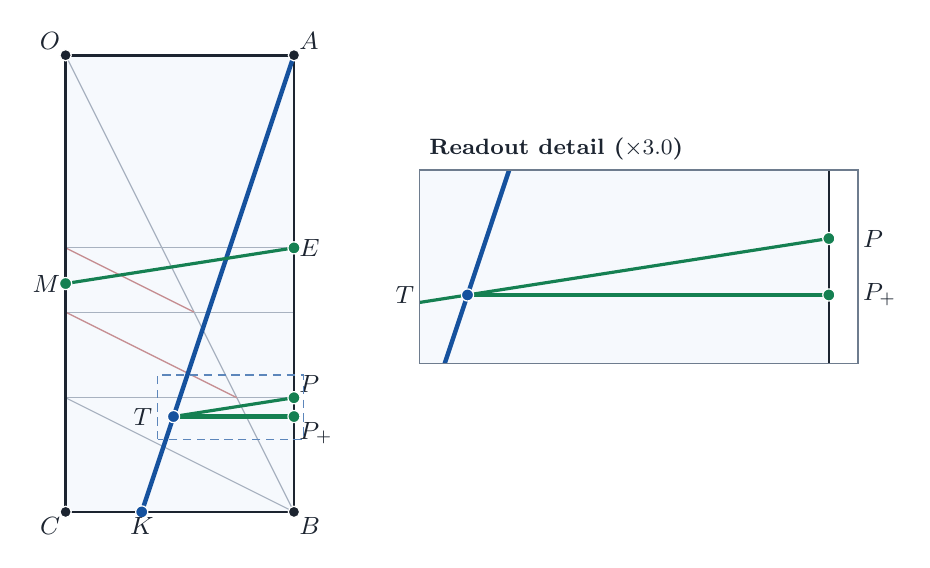
\begin{tikzpicture}[scale=1.45]
\fill[rectbg] (0.0000,0.0000) rectangle (2.0000,4.0000);
\draw[chain] (0.0000,4.0000)--(2.0000,0.0000);
\draw[chain] (0.0000,1.0000)--(2.0000,0.0000);
\draw[chain] (0,1.0000)--(2.0,1.0000);
\draw[chain] (0,1.7500)--(2.0,1.7500);
\draw[chain] (0,2.3125)--(2.0,2.3125);
\draw[chainpar] (1.5000,1.0000)--(0.0000,1.7500);
\draw[chainpar] (1.1250,1.7500)--(0.0000,2.3125);
\draw[rect] (0.0000,0.0000) rectangle (2.0000,4.0000);
\draw[support] (2.0000,4.0000)--(0.6667,0.0000);
\draw[transport] (0.0000,2.0000)--(2.0000,2.3125);
\draw[transport] (2.0000,1.0000)--(0.9451,0.8352);
\draw[transport,line width=1.65pt] (0.9451,0.8352)--(2.0000,0.8352);
\node[lab,above left] at (0.0000,4.0000) {$O$};
\node[lab,above right] at (2.0000,4.0000) {$A$};
\node[lab,below left] at (0.0000,0.0000) {$C$};
\node[lab,below right] at (2.0000,0.0000) {$B$};
\node[pt] at (0.0000,4.0000) {};
\node[pt] at (2.0000,4.0000) {};
\node[pt] at (0.0000,0.0000) {};
\node[pt] at (2.0000,0.0000) {};
\node[pttrans] at (0.0000,2.0000) {};
\node[pttrans] at (2.0000,2.3125) {};
\node[pttrans] at (2.0000,1.0000) {};
\node[ptsupp] at (0.9451,0.8352) {};
\node[pttrans] at (2.0000,0.8352) {};
\node[lab,left] at (0.0000,2.0000) {$M$};
\node[lab,right] at (2.0000,2.3125) {$E$};
\node[lab,above right] at (2.0000,1.0000) {$P$};
\node[lab,below right] at (2.0000,0.8352) {$P_+$};
\node[ptsupp] at (0.6667,0.0000) {};
\node[lab,below] at (0.6667,0.0000) {$K$};
\draw[aux,supp!70] (0.8051,0.6352) rectangle (2.0840,1.2000);
\node[lab,left] at (0.8051,0.8352) {$T$};
\begin{scope}[shift={(0.6848,-0.6055)},scale=3.0]
\begin{scope}
\clip (0.8051,0.6352) rectangle (2.0840,1.2000);
\fill[white] (0.8051,0.6352) rectangle (2.0840,1.2000);
\fill[rectfill] (0.8051,0.6352) rectangle (2.0,1.2000);
\draw[rect] (2.0,-0.3648)--(2.0,2.2000);
\draw[support] (2.0000,4.0000)--(0.6667,0.0000);
\draw[transport] (2.0000,1.0000)--(-3.0000,0.2188);
\draw[transport,line width=1.65pt] (0.9451,0.8352)--(2.0000,0.8352);
\node[pttrans] at (2.0000,1.0000) {};
\node[ptsupp] at (0.9451,0.8352) {};
\node[pttrans] at (2.0000,0.8352) {};
\end{scope}
\draw[line width=0.65pt,slatec] (0.8051,0.6352) rectangle (2.0840,1.2000);
\node[lab,right] at (2.0840,1.0000) {$P$};
\node[lab,right] at (2.0840,0.8352) {$P_+$};
\node[lab,left] at (0.8051,0.8352) {$T$};
\node[font=\footnotesize\bfseries,text=ink,anchor=south west] at (0.8051,1.2000) {Readout detail ($\times3.0$)};
\end{scope}
\end{tikzpicture}%
}

\newcommand{\figAD}{%
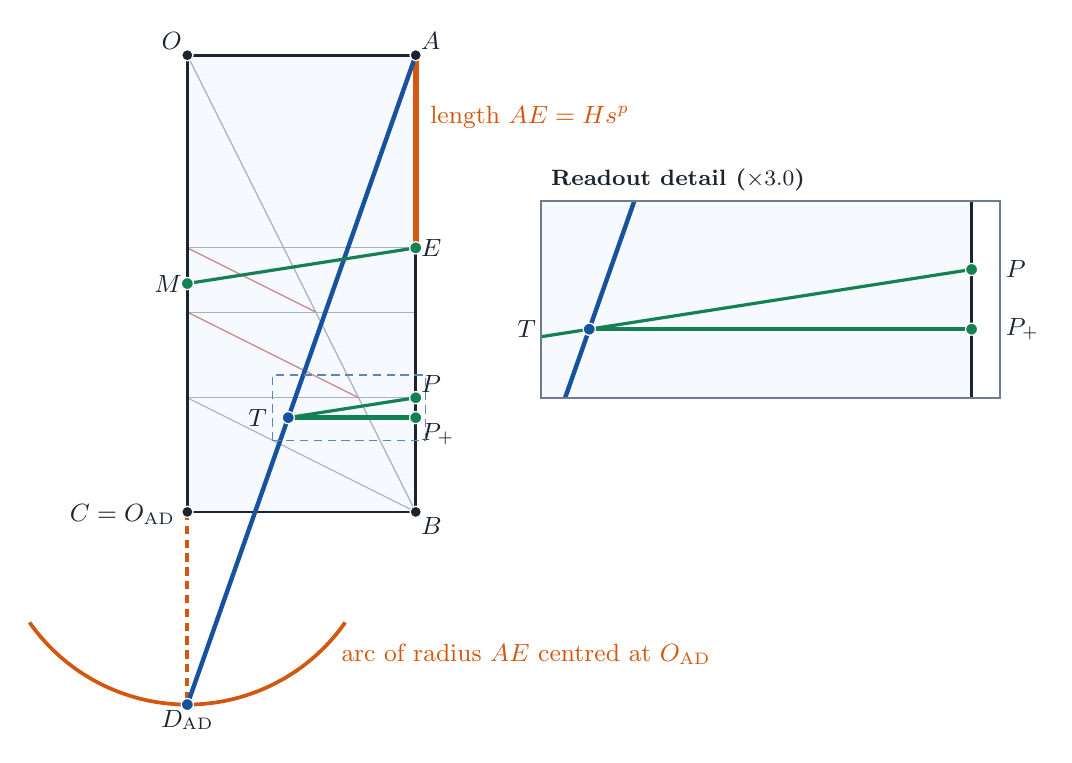
\begin{tikzpicture}[scale=1.45]
\fill[rectbg] (0.0000,0.0000) rectangle (2.0000,4.0000);
\draw[chain] (0.0000,4.0000)--(2.0000,0.0000);
\draw[chain] (0.0000,1.0000)--(2.0000,0.0000);
\draw[chain] (0,1.0000)--(2.0,1.0000);
\draw[chain] (0,1.7500)--(2.0,1.7500);
\draw[chain] (0,2.3125)--(2.0,2.3125);
\draw[chainpar] (1.5000,1.0000)--(0.0000,1.7500);
\draw[chainpar] (1.1250,1.7500)--(0.0000,2.3125);
\draw[rect] (0.0000,0.0000) rectangle (2.0000,4.0000);
\draw[accent] (0.0000,0.0000) ++(215:1.6875) arc (215:325:1.6875);
\draw[accent,densely dashed] (0.0000,0.0000)--(0.0000,-1.6875);
\draw[accent,line width=2.2pt] (2.0000,4.0000)--(2.0000,2.3125);
\draw[support] (2.0000,4.0000)--(0.0000,-1.6875);
\draw[transport] (0.0000,2.0000)--(2.0000,2.3125);
\draw[transport] (2.0000,1.0000)--(0.8837,0.8256);
\draw[transport,line width=1.65pt] (0.8837,0.8256)--(2.0000,0.8256);
\node[lab,above left] at (0.0000,4.0000) {$O$};
\node[lab,above right] at (2.0000,4.0000) {$A$};
\node[lab,anchor=east] at (-0.06,-0.02) {$C=O_{\mathrm{AD}}$};
\node[lab,below right] at (2.0000,0.0000) {$B$};
\node[pt] at (0.0000,4.0000) {};
\node[pt] at (2.0000,4.0000) {};
\node[pt] at (0.0000,0.0000) {};
\node[pt] at (2.0000,0.0000) {};
\node[pttrans] at (0.0000,2.0000) {};
\node[pttrans] at (2.0000,2.3125) {};
\node[pttrans] at (2.0000,1.0000) {};
\node[ptsupp] at (0.8837,0.8256) {};
\node[pttrans] at (2.0000,0.8256) {};
\node[lab,left] at (0.0000,2.0000) {$M$};
\node[lab,right] at (2.0000,2.3125) {$E$};
\node[lab,above right] at (2.0000,1.0000) {$P$};
\node[lab,below right] at (2.0000,0.8256) {$P_+$};
\node[ptsupp] at (0.0000,-1.6875) {};
\node[lab,below] at (0.0000,-1.6875) {$D_{\mathrm{AD}}$};
\node[lab,acc,anchor=west] at (2.0800,3.4562) {length $AE=Hs^p$};
\node[lab,acc,anchor=west] at (1.3,-1.25) {arc of radius $AE$ centred at $O_{\mathrm{AD}}$};
\draw[aux,supp!70] (0.7437,0.6256) rectangle (2.0840,1.2000);
\node[lab,left] at (0.7437,0.8256) {$T$};
\begin{scope}[shift={(0.8688,-0.8767)},scale=3.0]
\begin{scope}
\clip (0.7437,0.6256) rectangle (2.0840,1.2000);
\fill[white] (0.7437,0.6256) rectangle (2.0840,1.2000);
\fill[rectfill] (0.7437,0.6256) rectangle (2.0,1.2000);
\draw[rect] (2.0,-0.3744)--(2.0,2.2000);
\draw[support] (2.0000,4.0000)--(0.0000,-1.6875);
\draw[transport] (2.0000,1.0000)--(-3.0000,0.2188);
\draw[transport,line width=1.65pt] (0.8837,0.8256)--(2.0000,0.8256);
\node[pttrans] at (2.0000,1.0000) {};
\node[ptsupp] at (0.8837,0.8256) {};
\node[pttrans] at (2.0000,0.8256) {};
\end{scope}
\draw[line width=0.65pt,slatec] (0.7437,0.6256) rectangle (2.0840,1.2000);
\node[lab,right] at (2.0840,1.0000) {$P$};
\node[lab,right] at (2.0840,0.8256) {$P_+$};
\node[lab,left] at (0.7437,0.8256) {$T$};
\node[font=\footnotesize\bfseries,text=ink,anchor=south west] at (0.7437,1.2000) {Readout detail ($\times3.0$)};
\end{scope}
\end{tikzpicture}%
}

\newcommand{\figProjective}{%
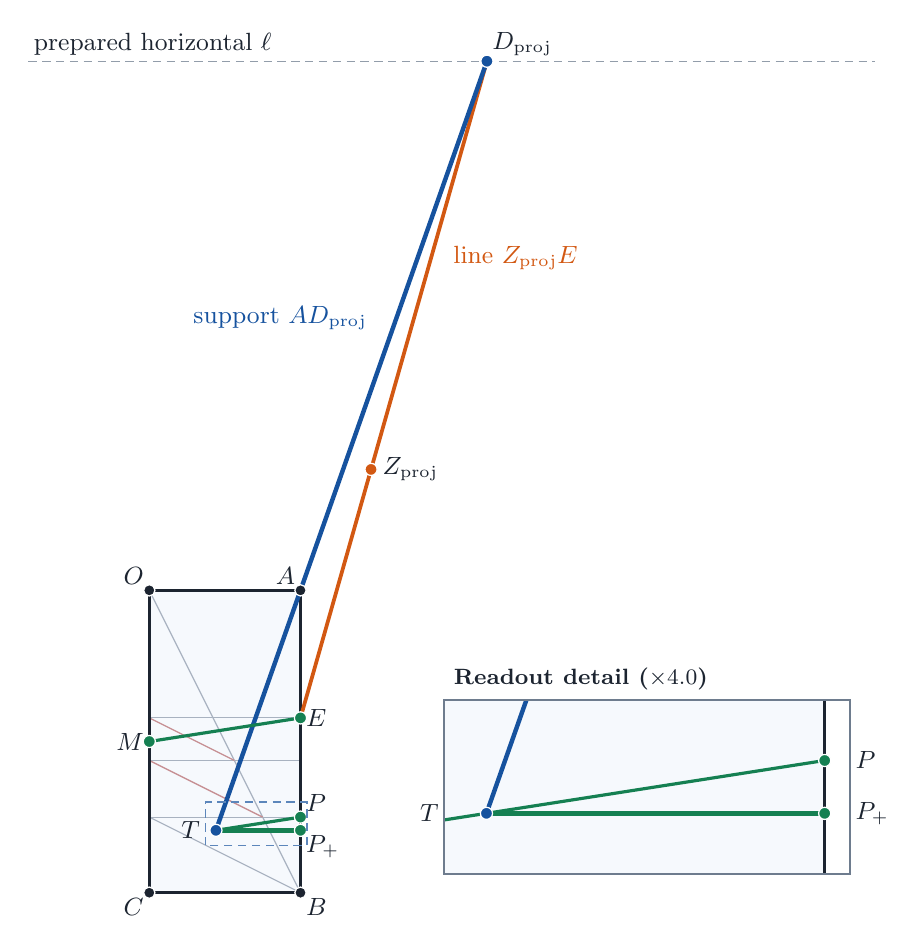
\begin{tikzpicture}[scale=0.96]
\draw[aux] (-1.6,11.0000)--(9.6,11.0000);
\node[lab,anchor=south west] at (-1.6,11.0000) {prepared horizontal $\ell$};
\fill[rectbg] (0.0000,0.0000) rectangle (2.0000,4.0000);
\draw[chain] (0.0000,4.0000)--(2.0000,0.0000);
\draw[chain] (0.0000,1.0000)--(2.0000,0.0000);
\draw[chain] (0,1.0000)--(2.0,1.0000);
\draw[chain] (0,1.7500)--(2.0,1.7500);
\draw[chain] (0,2.3125)--(2.0,2.3125);
\draw[chainpar] (1.5000,1.0000)--(0.0000,1.7500);
\draw[chainpar] (1.1250,1.7500)--(0.0000,2.3125);
\draw[rect] (0.0000,0.0000) rectangle (2.0000,4.0000);
\draw[accent] (2.0000,2.3125)--(4.4664,11.0000);
\draw[support] (0.8814,0.8252)--(4.4664,11.0000);
\draw[transport] (0.0000,2.0000)--(2.0000,2.3125);
\draw[transport] (2.0000,1.0000)--(0.8814,0.8252);
\draw[transport,line width=1.65pt] (0.8814,0.8252)--(2.0000,0.8252);
\node[lab,above left] at (0.0000,4.0000) {$O$};
\node[lab,above left] at (2.0000,4.0000) {$A$};
\node[lab,below left] at (0.0000,0.0000) {$C$};
\node[lab,below right] at (2.0000,0.0000) {$B$};
\node[pt] at (0.0000,4.0000) {};
\node[pt] at (2.0000,4.0000) {};
\node[pt] at (0.0000,0.0000) {};
\node[pt] at (2.0000,0.0000) {};
\node[pttrans] at (0.0000,2.0000) {};
\node[pttrans] at (2.0000,2.3125) {};
\node[pttrans] at (2.0000,1.0000) {};
\node[ptsupp] at (0.8814,0.8252) {};
\node[pttrans] at (2.0000,0.8252) {};
\node[lab,left] at (0.0000,2.0000) {$M$};
\node[lab,right] at (2.0000,2.3125) {$E$};
\node[lab,above right] at (2.0000,1.0000) {$P$};
\node[lab,below right] at (2.0000,0.8252) {$P_+$};
\node[ptacc] at (2.9333,5.6000) {};
\node[ptsupp] at (4.4664,11.0000) {};
\node[lab,right] at (3.0133,5.6000) {$Z_{\mathrm{proj}}$};
\node[lab,above right] at (4.4664,11.0000) {$D_{\mathrm{proj}}$};
\node[lab,acc,anchor=west] at (3.95,8.4) {line $Z_{\mathrm{proj}}E$};
\node[lab,supp,anchor=east] at (2.95,7.6) {support $AD_{\mathrm{proj}}$};
\draw[aux,supp!70] (0.7414,0.6252) rectangle (2.0840,1.2000);
\node[lab,left] at (0.7414,0.8252) {$T$};
\begin{scope}[shift={(0.9345,-2.2509)},scale=4.0]
\begin{scope}
\clip (0.7414,0.6252) rectangle (2.0840,1.2000);
\fill[white] (0.7414,0.6252) rectangle (2.0840,1.2000);
\fill[rectfill] (0.7414,0.6252) rectangle (2.0,1.2000);
\draw[rect] (2.0,-0.3748)--(2.0,2.2000);
\draw[support] (0.8814,0.8252)--(4.4664,11.0000);
\draw[transport] (2.0000,1.0000)--(-3.0000,0.2188);
\draw[transport,line width=1.65pt] (0.8814,0.8252)--(2.0000,0.8252);
\node[pttrans] at (2.0000,1.0000) {};
\node[ptsupp] at (0.8814,0.8252) {};
\node[pttrans] at (2.0000,0.8252) {};
\end{scope}
\draw[line width=0.65pt,slatec] (0.7414,0.6252) rectangle (2.0840,1.2000);
\node[lab,right] at (2.0840,1.0000) {$P$};
\node[lab,right] at (2.0840,0.8252) {$P_+$};
\node[lab,left] at (0.7414,0.8252) {$T$};
\node[font=\footnotesize\bfseries,text=ink,anchor=south west] at (0.7414,1.2000) {Readout detail ($\times4.0$)};
\end{scope}
\end{tikzpicture}%
}

\newcommand{\figMB}{%
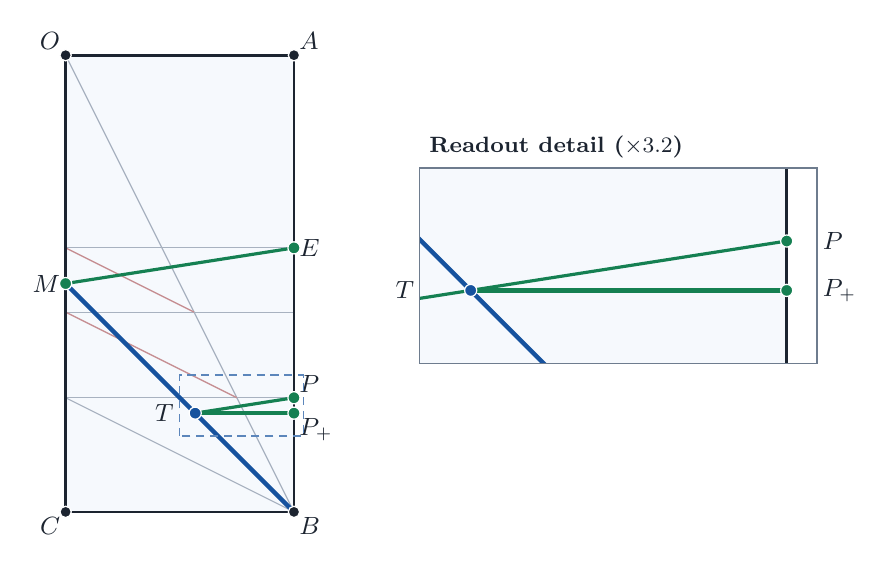
\begin{tikzpicture}[scale=1.45]
\fill[rectbg] (0.0000,0.0000) rectangle (2.0000,4.0000);
\draw[chain] (0.0000,4.0000)--(2.0000,0.0000);
\draw[chain] (0.0000,1.0000)--(2.0000,0.0000);
\draw[chain] (0,1.0000)--(2.0,1.0000);
\draw[chain] (0,1.7500)--(2.0,1.7500);
\draw[chain] (0,2.3125)--(2.0,2.3125);
\draw[chainpar] (1.5000,1.0000)--(0.0000,1.7500);
\draw[chainpar] (1.1250,1.7500)--(0.0000,2.3125);
\draw[rect] (0.0000,0.0000) rectangle (2.0000,4.0000);
\draw[support] (0.0000,2.0000)--(2.0000,0.0000);
\draw[transport] (0.0000,2.0000)--(2.0000,2.3125);
\draw[transport] (2.0000,1.0000)--(1.1351,0.8649);
\draw[transport,line width=1.65pt] (1.1351,0.8649)--(2.0000,0.8649);
\node[lab,above left] at (0.0000,4.0000) {$O$};
\node[lab,above right] at (2.0000,4.0000) {$A$};
\node[lab,below left] at (0.0000,0.0000) {$C$};
\node[lab,below right] at (2.0000,0.0000) {$B$};
\node[pt] at (0.0000,4.0000) {};
\node[pt] at (2.0000,4.0000) {};
\node[pt] at (0.0000,0.0000) {};
\node[pt] at (2.0000,0.0000) {};
\node[pttrans] at (0.0000,2.0000) {};
\node[pttrans] at (2.0000,2.3125) {};
\node[pttrans] at (2.0000,1.0000) {};
\node[ptsupp] at (1.1351,0.8649) {};
\node[pttrans] at (2.0000,0.8649) {};
\node[lab,left] at (0.0000,2.0000) {$M$};
\node[lab,right] at (2.0000,2.3125) {$E$};
\node[lab,above right] at (2.0000,1.0000) {$P$};
\node[lab,below right] at (2.0000,0.8649) {$P_+$};
\draw[aux,supp!70] (0.9951,0.6649) rectangle (2.0840,1.2000);
\node[lab,left] at (0.9951,0.8649) {$T$};
\begin{scope}[shift={(-0.0844,-0.8276)},scale=3.2]
\begin{scope}
\clip (0.9951,0.6649) rectangle (2.0840,1.2000);
\fill[white] (0.9951,0.6649) rectangle (2.0840,1.2000);
\fill[rectfill] (0.9951,0.6649) rectangle (2.0,1.2000);
\draw[rect] (2.0,-0.3351)--(2.0,2.2000);
\draw[support] (0.0000,2.0000)--(2.0000,0.0000);
\draw[transport] (2.0000,1.0000)--(-3.0000,0.2188);
\draw[transport,line width=1.65pt] (1.1351,0.8649)--(2.0000,0.8649);
\node[pttrans] at (2.0000,1.0000) {};
\node[ptsupp] at (1.1351,0.8649) {};
\node[pttrans] at (2.0000,0.8649) {};
\end{scope}
\draw[line width=0.65pt,slatec] (0.9951,0.6649) rectangle (2.0840,1.2000);
\node[lab,right] at (2.0840,1.0000) {$P$};
\node[lab,right] at (2.0840,0.8649) {$P_+$};
\node[lab,left] at (0.9951,0.8649) {$T$};
\node[font=\footnotesize\bfseries,text=ink,anchor=south west] at (0.9951,1.2000) {Readout detail ($\times3.2$)};
\end{scope}
\end{tikzpicture}%
}

